\documentclass{sig-alternate}
\usepackage{enumitem}
\usepackage{xspace}
\usepackage{caption}
\usepackage{subfig}
\usepackage{paralist, tabularx}

\begin{document}
\newcommand{\nifty}{\textsf{Papyr}\xspace}

\conferenceinfo{DEV}{'14 San Jose, California USA}
\title{Papyr: Automatically Generating ``Smart" Paper Tools for Low-resource Settings}
\author{}
\maketitle

\begin{abstract}
% For low-resource organizations working in developing regions, paper remains the default information medium of choice. 
%is it by choice or by necessity% 
Despite the recent push toward leveraging information and communication technologies (ICTs) for replacing paper-based tasks, there remain many barriers to designing deployable and appropriate technical solutions that replace paper.
%i dont like this%
%also what tasks do you mean when you say "these tasks"%
As a result, paper tools such as forms, charts, and graphs continue to be widely used in low-resource organizations working in developing regions.
Unfortunately, existing paper tools are often designed to be out of reach for end-users and depend on intermediaries to input data and interpret information. 
We apply ideas from computability and human-computer interaction to design a system to automatically generate paper tools that provide immediate computation, visual feedback, and independence from both ICTs and intermediaries at the point of use. 
\nifty is a system that is easy to use and allows low-resource organizations to quickly transform data tracking or information dissemination requirements into printable ``smart'' paper tools. 
%maybe we should come up with a different phrase from "data tracking" and "information dissemination"
In this paper, we explore how paper tools are currently being used by organizations in Ghana, explore the design space for smart paper tools, and describe \nifty's design and implementation.

\end{abstract}

% \category{}{}{}
% \category{}{}{}
% \terms{}
% \keywords{}

%%%%%%%%%%%%%%%%%%%%%%%%%%%%%%%%%%%%%%%%%%%%%%%%%%%%%

\section{Introduction}

Even as computing devices proliferate, often with the singularly ambitious goal of eliminating paper from a given ecosystem, the fact that paper continues to be pervasive in professional and personal spaces is undeniable. Paper is light, low-cost, familiar, accessible, easy to use, intuitive to manipulate, and convenient to distribute \cite{sellen1997,sellen2002,johnson1993}. Moreover, in low-resource settings where technology infrastructure, such as stable electricity, cutting-edge computer hardware and software, and skilled human capital, is deficient, paper is an obvious choice because it can accomplish many of the same tasks that computers can, including tracking, recording, and look-up. Furthermore, generations of paper-based organizational and end-user tasks have ensured that national regulations, at least in most of the developing world, seek compliance with paper-based record keeping rules. The enduring legacy of paper, especially amongst current paper-based workflows, provides inertia against switching to more technically intensive replacements. It is little wonder then that paper continues to be the information medium of choice in many low-resource organizations providing community health and microfinance services in the developing world.

Still, paper is not without its constraints. The most pertinent drawbacks of paper when compared to information and communication technology (ICT) alternatives is its limited ability to manipulate data once it has been inscribed, lack of ``computational output'', and difficulty in digitization. Electronic media that is designed and built to replace paper possesses an almost inverse profile of strengths, but, in being unable to capitalize on paper's more accessible and tangible properties, also has opposing constraints \cite{johnson1993}. Can paper itself be designed to overcome some of these limitations? Can paper, for instance, make its static content dynamic? Or, perhaps, even more ambitiously, can paper provide computational feedback to its end users? 

There already exist many examples of what we call ``smart paper'' that demonstrate how these lofty objectives are in fact possible. Paper graphs, for instance, can provide computational feedback. One example is the nomograph, a graphical calculating device that has three scales to represent a three-variable equation. By plotting along these scales using just a pen, one can determine their ideal body mass, to give one illustration, by locating their results within the ``overweight", ``desirable", or ``underweight" categories, while accounting for any gender differences \cite{thomas1976}. The partograph, another example, is a graphical tool that can provide predictive feedback to doctors or midwives throughout the progress of labour\cite{who1988}. The partograph, in fact, is an especially interesting example of ``smart paper" given its popularity in low-resource settings \cite{fawole2009, umezulike1999}. It is a paper tool that is cost-effective and accessible, a tool that when coupled with well-defined protocols and appropriate instruction has been shown to demonstrate distinct benefits in the developing world \cite{fahdy2005, pettersson2000}.

These examples of ``smart" paper tools indicate a particularly compelling research problem of leveraging paper's many useful properties and developing more standalone tools, while simultaneously validating their usefulness in low-resource settings where paper is cheaper, more familiar, and more accessible than its technology counterparts. Our study addresses this research problem with the following contributions:

\begin{compactitem}

  \item Needs assessment of low-resource settings for microfinance and health in Ghana through an appraisal of existing paper artifacts and understanding of information gaps. (Section~\ref{sec:exploring-paper}).
  \item Development of ``smart'' paper tools that are pushing the boundaries of paper and exploring how paper can contribute to existing processes, especially with low-literate populations in mind (Section~\ref{sec:exploring-paper}).
  \item Discovery of basic design principles that highlight the constraints of paper and user interaction with ``smart'' paper tools (Section~\ref{sec:constraints}).
  \item Construction of \nifty, a system for intermediaries from low-resource organizations to automatically generate ``smart'' paper tools by simply defining their tasks and their associated paramters. The intermediary can then select from suggestions based on resources available and capabilities of the end-user to print and construct the paper tools based on the resources available (Section~\ref{sec:system-desc}). 

\end{compactitem}

% We believe \nifty is an unusual but appropriate marriage between paper and technology for developing contexts: a computer is used to support the organization's design of context-specific paper tools, but the produced paper tools require no ICT support or leverage at the end user. [something else]

% To address this research problem, we conducted a needs assessment in low-resource settings in Ghana that sought to appraise existing paper artifacts in the health and microfinance contexts. Based on our needs assessment, we found that though paper tools are fairly ubiquitous, they often require intermediaries for use and interpretation. From our findings, we design paper tools that provided direct and immediate computational or visual feedback for end users. These tools are specifically designed for low-literate populations, ensuring that the need for any textual input was alleviated as much as was possible. We also develop more general smart paper tools that are not grounded in context-specific constraints to focus more on exploring, and perhaps, exploiting, the many properties of paper for a broader range of problems.
%We elaborate on this process in Section~\ref{sec:exploring-paper}, the ``Exploring Paper" section.

%Based on the lessons we learned from our needs assessment
%, as discussed in Sections~\ref{sec:abstraction} and \ref{sec:constraints}, 
% From our exploration we abstracted the problem in order to develop, \nifty, a system for \emph{intermediaries} in low-resource organizations to automatically generate smart paper tools by simply defining their tasks and their associated parameters. Given these inputs \nifty produces suggestions of smart paper tools for the intermediary to select based on the resources available and capabilities of the end user. The intermediary can then print and construct the paper tool according to the instructions provided by \nifty and then distribute the tool to \emph{end users}. We believe \nifty is an unusual but appropriate marriage between paper and technology for developing contexts: a computer is used to support the organization's design of context-specific paper tools, but the produced paper tools require no ICT support or leverage at the end user. For clarity, throughout this paper we refer to the ``end user'' as the user who uses the paper tools themselves, and the ``user'' as the low-resource organization's intermediary who uses \nifty to create paper tools.
%The system is described in Section.

%We make two important design decisions at the onset of developing \nifty. First, in order to deliver smart paper tools to potentially low-literate users with limited exposure to computers and other forms of technology, it is necessary that a more skilled intermediary or a representative from a particular organizational setting (such as a hospital or an MFI) that is familiar with the context defines the input parameters on \nifty and generates the required paper tools. Therefore, \nifty was designed to be used by these intermediaries, whereas the paper tools were generated to be used by the customers of the MFI or the patients at the clinic. Second, the decision to introduce technology was taken to develop an infrastructure that could support the construction and dissemination of these smart paper tools on a larger scale. Therefore, a computer is necessary to support the centralized production and distribution of context-specific paper tools. This integration points to an unusual marriage of paper and technology, where the beneficial properties of paper, such as its tangibility, flexibility, affordability, and accessibility are completely preserved, and where the technology is required only until the point of distribution. The actual assembly and use of the paper outputs requires no technical support or leverage. 

%We describe this system, NiftyPaper, in detail in Section~\ref{sec:system-desc}. Finally, we conclude with the ``discussion and conclusion" in section~\ref{sec:discussion} and point to directions for ``future work" in Section~\ref{sec:future-work}. 

%%%%%%%%%%%%%%%%%%%%%%%%%%%%%%%%%%%%%%%%%%%%%%%%%%%%%

\section{Related Work}
The oldest vision for the integration of paper and computers may perhaps be the conceptualization of Digital Desk \cite{wellner1993}. Digital Desk sought to more seamlessly integrate paper and digital documents by coupling paper with graphics projections, enabling interactions with paper in a way that allows for the completion of typical computing tasks. Still, the most recognizable paper-computer relationship is manifest in the printer itself \cite{qi2010}. However, when it comes to existing work that is directly related to this study, the printer is mostly used as a means to generate interesting paper artifacts that is an integration of computation and paper. For instance, the printer has been leveraged to generate 3-D shapes or pop-up sculptures \cite{eisenberg1997, hendrix2005}. Similarly, for this study, we rely on the printer to generate standalone, smart paper tools that provide augmented computational and visual feedback.

The emerging field of ``paper computing" is a step in the direction of more seamlessly integrating paper's inherent, constructive affordances with the computational power of technology, and in doing so, rejecting the very notion of a ``paperless world" \cite{kaplan2010}. Current work includes augmented paper documents, where paper sheets are digitally enhanced through the use of printed visual markers such as QR codes \cite{kaplan2010} or through the inscription of digital notes via specialized devices \cite{anoto, pietrzak2010}. Still other applications include leveraging paper itself as an interface to computer applications; these interfaces may be paper-based \cite{bonnard2010, portocarrero2010} or paper-like \cite{qi2010, coelho2009}. In addition, there are various examples of paper computing tools that have been designed specifically for the developing world. For example, CAM, a user interface toolkit, uses a mobile phone with a camera to record and store data from paper logs in rural microfinance groups in India \cite{parikh2006}. Digital Slate, an example of a paper-like interface, is a low-cost electronic slate that allows for pen-to-paper writing motion to capture data in savings groups in India \cite{ratan2010}. Shreddr is another example of paper to electronic data conversion technology that can be used in any low-resource organization that remains heavily dependent on paper\cite{chen2012}. However, these paper computing tools that have been designed for the developing world almost exclusively focus on capturing and converting data, while ignoring a range of other tasks.

In general, in the best-case scenarios for paper computing tools, the constructive benefits of paper and technology are leveraged equally. In the worst-case scenarios, as is usually the case, these instances of the integration of paper and technology almost always end up compromising on paper's low-cost and easy availability, or underutilizing its computational power. In contrast, this project focuses instead almost exclusively on exploiting and preserving the valuable affordances of paper by bringing in technology to furnish the \emph{supporting} infrastructure to generate smart paper tools. This unique stance is justified in low-resource settings where paper is inexpensive, easily accessible, and familiar, thereby mitigating resource, training, and infrastructure costs \cite{chen2012}.


%%%%%%%%%%%%%%%%%%%%%%%%%%%%%%%%%%%%%%%%%%%%%%%%%%%%%

\section{Exploring Paper}
\label{sec:exploring-paper}

For this project we focus on specific problems within the health and microfinance contexts. After establishing the problem space, reviewing the related work, and identifying real-world problems in low-resource settings where paper is already deeply rooted and in constant use, we held several brainstorming sessions to ambitiously explore the range of computational and visual feedback that paper in and of itself could provide. We then explored how paper was being used in the health and microfinance contexts at field sites in Ghana to assess how paper is currently being used. Finally, we designed several improvements to existing paper tools and iterated on our designs with real end users.

\subsection{What Can Paper Do?}

%Our brainstorming sessions were accompanied with needs assessment studies in parallel where we visited low-income populations (usually areas with low-income housing options, or wholesale market places) within Accra and conducted informal interviews with people regarding their health and financial practices, and any tools (paper or otherwise) they might already be using to support these practices. This qualitative understanding helped ground our ideas in a real-world context to justify their continued assessment and to focus our scope. 
The primary goal of these preliminary brainstorming sessions was to push the boundaries of what ``smart paper" could accomplish. In other words, how could we re-design paper in a way that makes it somehow better? Here, we describe a small subset of the ``smart-paper" tools we designed in our brainstorming sessions.

\subsubsection{The Subtraction Band}

The subtraction band gives the difference of numbers. The base is made of stiff paper, plastic, cardboard, or other material that could support two narrow slits through which a closed paper loop could be smoothly slid and rotated. Figure \ref{fig:band} is a representation of this tool where the numbered upper region is the base in reference to which the paper loop, or darker region, would move.

To take a simple example, we shaded ten boxes on the number line on the base. We now want to subtract ``3" from ``10" (Figure~\ref{fig:band-init}). We locate ``3" on the number line and remove the stickers until that point. After this slide the paper band to the left such that the first shaded cell moves back to ``1". We can now see that the result is ``7" (Figure~\ref{fig:band-final}). Alternatively, if materials are available, shading cells could be replaced with sticking stickers.

\begin{figure}%
    \centering
    \subfloat[Initial]{{\label{fig:band-init}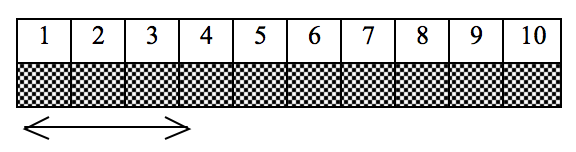
\includegraphics[width=.8\linewidth]{img/band-init.png} }}%
    \qquad
    \subfloat[Final]{{\label{fig:band-final}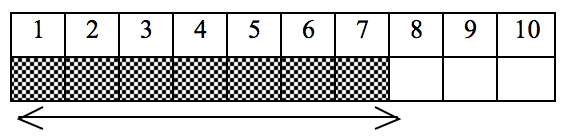
\includegraphics[width=.8\linewidth]{img/band-final.png} }}%
    \caption{Subtraction band initial and final state.}%
    \label{fig:band}%
\end{figure}

\subsubsection{The Addition By Matching Tool}

The addition by matching tool calculates the sum as well as compares and matches analogous variables. Again, the base would be made of stiff paper, plastic, cardboard, or other material that would support two narrow slits through which a paper strip could be smoothly slid up or down. Figure \ref{fig:add} is a representation of this tool, where the axes indicate the base in which each separate strip, or column, would move in relation to.

Income inflows for low-income populations typically engaged in the informal labour market are irregular and variable, accumulated through a variety of financial instruments such as money earned through different jobs and money borrowed through different sources of credit. This tool can be used to compare income and expenses, for instance, and determine when income-expenses can be met or matched or when one exceeds the other. To do this, we first shade in the requisite number of 100 cedi\footnote{local currency corresponding to roughly 0.28 USD per cedi at the time of writing} cells to fill up the projected income and expenses column on ``Day 1". We then fill in cells in the income and expenses column on ``Day 2", starting from the point where income and expenses leveled out, respectively, on the previous day. This is repeated for every successive day. At this point, the tool is able to tell the user when expenses exceed income. 

In this example, user estimates that the incomes for the first day will be around 200 cedi, shading cells to fill that amount. The user then estimates that on the second day, income will be approximately 300 cedi. He or she would then fill the cells from the bottom up to the 300 cedi point and then shift the band so that the starting point of the shaded cells is at the point in which they left off, or at the 200 cedi mark. The resulting configuration can be seen in Figure~\ref{fig:add-init}. The user is now able to tell that over the two days, the income has accumulated to 500 cedis. And after populating the expenses columns in a similar manner on the tool, the user can see that expenses exceed income on ``Day 1", income exceeds expenses on ``Day 2", and they match on ``Day 3". The tool also indicates how much money has accumulated at any given time, by checking the scale on the left.
 
While tracking income-expenses, if there is an unexpected expense unit that is introduced on ``Day 1" (represented by the red cell in Figure \ref{fig:add-final}), then the successive stacks of expenses must be readjusted. This is achieved by sliding the paper strips representing expenses on ``Day 2" and ``Day 3" one unit up. The tool is therefore able to readjust to match the dynamic nature of money flow for low-income populations.

\begin{figure}%
    \centering
    \subfloat[Initial]{{\label{fig:add-init}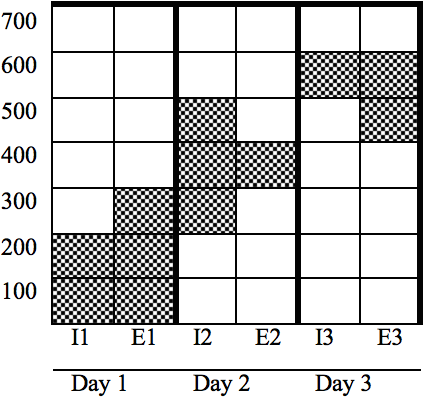
\includegraphics[width=.43\linewidth]{img/add-init.png} }}%
    \qquad
    \subfloat[Final]{{\label{fig:add-final}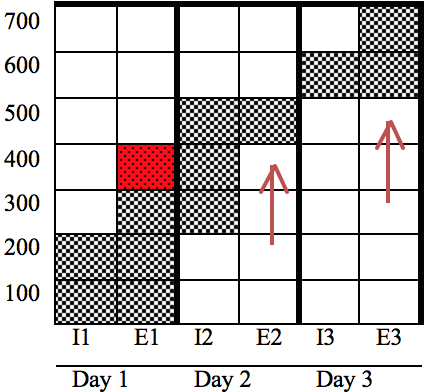
\includegraphics[width=.43\linewidth]{img/add-final.png} }}%
    \caption{Addition and matching tool initial and final state.}%
    \label{fig:add}%
\end{figure}

\subsubsection{Averages Tool}

We also developed a tool that could help estimate averages. Averages, for instance, can be particularly useful in calculating the length of a typical menstrual cycle in order to predict the length of future cycles. In its simplest form, a rolled strip of paper can be incrementally unrolled by a standard unit size to track each day the individual is not menstruating and then ripped or torn when menstruation occurs. 

When these strips of paper are layered up on top of each other, the thickest part of the strips would indicate where the average would be located. The next time the individual is unrolling the strips of paper, they can know where to anticipate their cycle to end. Additionally, the halfway point is a good approximation of when ovulation would occur. A similar process could be done with the strips of paper folded in half to have a rough estimate of when the individual is most fertile. 

Arranging these strips of paper next to each other would also give a good ``eyeball" estimate of the average, as seen in Figure~\ref{fig:avg-basic}. This could be enhanced with the use of a tool that lines up with shortest strip and the longest strip in the range of data points and, with springs or rubber bands attached to the middle mark, draws a line between the two to come up with an alternate means of estimating the average as seen in Figure~\ref{fig:avg-spring}. These two do not necessarily give a very accurate average, but each has its own strengths. 

Another potential design is taking thinner but sturdier strips of paper or string marked with standardized units. The strip is unrolled during the current cycle from the end of the last cycle and all of it is wound around two thin stiff rods, such as a pencil, the number of times that is the number of cycles. These can then be readjusted so that the strip comfortably spans the two rods in a way that results in equivalent sections for the number of cycles. A graphical depiction is seen in Figure~\ref{fig:avg-wrap}. This can give a fairly accurate estimation of average. However, there is a tradeoff because this is one of the prototypes that is the hardest to implement due to the need for very specific materials and complicated gestures.

\begin{figure}%
    \centering
    \subfloat[Basic]{{\label{fig:avg-basic}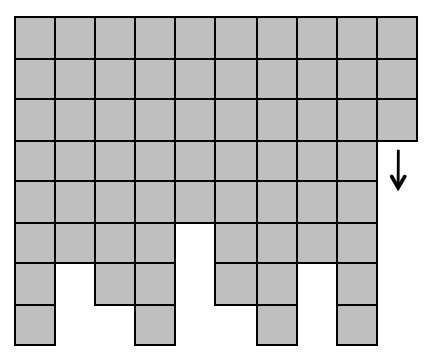
\includegraphics[width=.25\linewidth]{img/avg-basic.png} }}%
    \qquad
    \subfloat[Spring]{{\label{fig:avg-spring}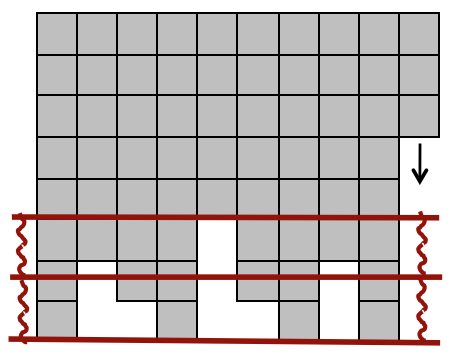
\includegraphics[width=.25\linewidth]{img/avg-spring.png} }}%
    \qquad
    \subfloat[Wrap]{{\label{fig:avg-wrap}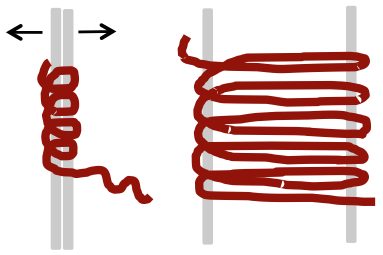
\includegraphics[width=.25\linewidth]{img/avg-wrap.png} }}%
    \caption{Different iterations of a tool to find averages.}%
    \label{fig:avg}
\end{figure}

\subsection{In the Field Design Iterations}

After our ideation sessions, we developed context-specific tools that were designed specifically to address any deficiencies in existing paper artifacts we observed. We conducted contextual inquiries in the domains of microfinance and public health in Accra, Tema, Dodowa, and Awutu-Senya in Ghana over a period of three weeks in July 2014. During this time, we observed the organizational settings, user practices, and existing paper artifacts. We briefly describe these artifacts, the tools we designed in response, and their testing and subsequent iterations during our time in the field.

\subsubsection{Susu Tracker}
% JAY: photo of existing susu tracker
We spent time with a microfinance institution (MFI) in Tema, observing their daily ``susu" (savings) operations. The susu process itself is straightforward. Clients deposit a standard susu deposit amount for 31 days, of which 30 days worth of accumulated sum is theirs to withdraw at any time and 1 days worth of deposit is the commission for the MFI. Therefore, the deposit that the customer made on the first day of a new cycle is immediately forfeited to the MFI as their commission. A standard paper passbook was used to record these transactions. The passbook provides the date on which a deposit was made, the amount deposited, and the running total up until 31 days. Therefore, if a customer had saved over multiple 31-day cycles without making any withdrawals, he or she would now have to add the accumulated sum per completed cycle, which would be a standard amount, plus any arbitrary amount for a partially completed cycle. Moreover, the passbook provides no commission information. More specifically, the running total for one cycle did not indicate to the user in any way that one day's worth of deposit would be immediately subtracted from the accumulated sum, should they choose to withdraw that amount.

After observing these deficiencies, we designed a tool that could give the customer this missing information. Most of the existing customers had low-literacy and arithmetic skills, so we decided to keep the input process as simple and straightforward as possible. One of the first iterations used a calendar layout along with a stack of stickers that had the running total and commission information denoted by a red sticker that accumulated in arithmetic progression every 31 days (Figure \ref{fig:susu-init}). After five design and usability testing iterations, our final susu tracker represented a simple passbook format (without stickers) where the dates and the running total were already printed out (retaining the commission information as before), and customers only had to mark or tick off the days on which they made a deposit using a pen or pencil (Figure \ref{fig:susu-final}).

\begin{figure}%
    \centering
    \subfloat[Initial]{{\label{fig:susu-init}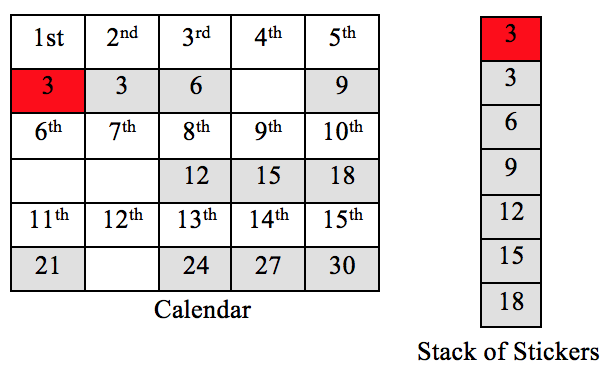
\includegraphics[width=.8\linewidth]{img/susu-init.png} }}%
    \qquad
    \subfloat[Final]{{\label{fig:susu-final}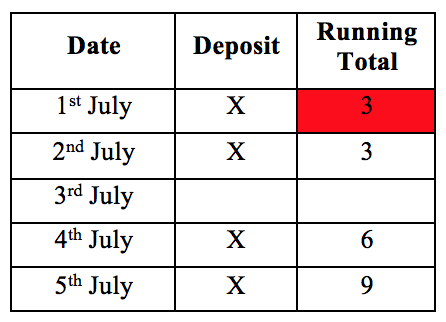
\includegraphics[width=.6\linewidth]{img/susu-final.png} }}%
    \caption{Susu tracker initial and final state.}%
    \label{fig:susu}%
\end{figure}

\subsubsection{Graph Reader}

At a government district and a children's hospital in the greater Accra region, we observed daily medical practices and conducted interviews with different doctors and nurses. We also interviewed medical professors and intermediaries, such as local community health volunteers. Through our interactions we learned that women are required to maintain two booklets before, during, and after pregnancy. One booklet was used to track the health of the mother, and the other, of the child. Unfortunately, the information contained in these booklets was presented in a very complicated manner, primarily to be used by trained medical personnel.

In the booklets there was a chart that mapped the age of the child over the weight of the child to determine whether the child is at a healthy weight-age balance based on the WHO regulations of child growth percentiles. This chart also tracks the child's weight over 24 months, accompanied by a legend to indicate the possible slopes between each of the points, and their implications (that is, points with a negative slope, or where the second dot is lower than the first, indicate that the child is losing weight and is in a danger zone). An adaptation of this legend can be seen in Figure~\ref{fig:graph-slope}. Through the interviews, we discovered that this information would in fact be relevant to the mothers. But given the confusing and esoteric presentation, it was inaccessible for those who did not know how to read graphs, and clunky to use for those who could read graphs. Therefore, we decided to develop a tool that would help individuals read this graphical information more easily.

To improve this tool for low-literate populations, the first challenge was finding a way pinpoint the location of the information of interest. Various ideas for tools were developed, including tabs that stretch to the numbers of interest on the graph and position the basic square viewfinder as seen in Figure~\ref{fig:graph-square}. Another idea was hollow strips that could be placed on the axes to point to a given region and would overlap to pinpoint the specific region in the center, as seen in Figure~\ref{fig:graph-strips}. However, based on design principles for low-literacy users and feedback from the needs assessment, we decided we not only needed to highlight the important regions but also to cover the information that is not needed. Therefore, we toyed around with overlapping and sliding pieces of paper and developed a tool that uses horizontal and vertical tabs to slide the region of emphasis in place. An example of this tool can be seen later in the paper in Figure~\ref{fig:graph-tool}.

Another design question was finding ways to compare two points with each other. This could involve something as basic as the slope comparison that the current child and maternal health records use. Or, this could use the viewfinder's space to compare the slope of two points. After feedback from nurses and doctors, the final iteration of the tool includes a viewfinder that compares points based on the quadrants they fall in, as seen in Figure~\ref{fig:graph-viewfinder}.

\begin{figure}%
    \centering
    \subfloat[Square]{{\label{fig:graph-square}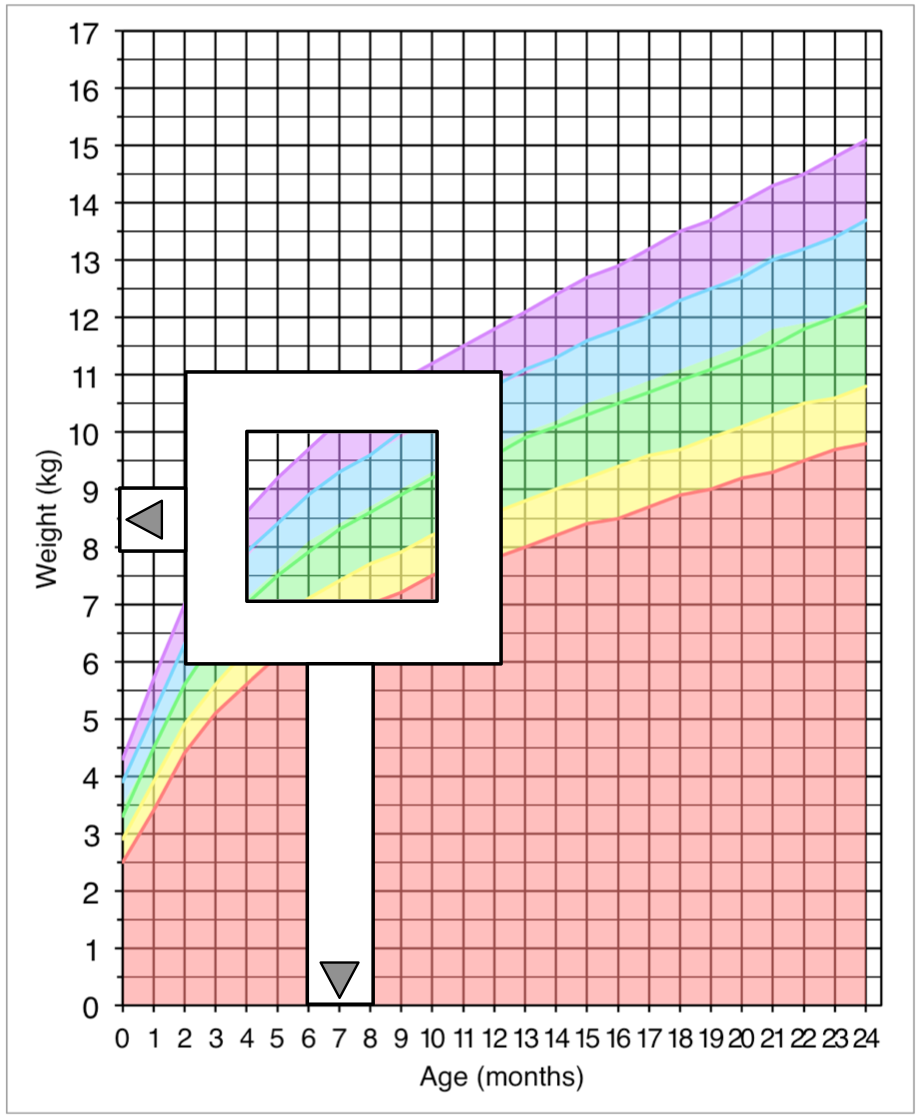
\includegraphics[width=.4\linewidth]{img/graph-square.png} }}%
    \qquad
    \subfloat[Strips]{{\label{fig:graph-strips}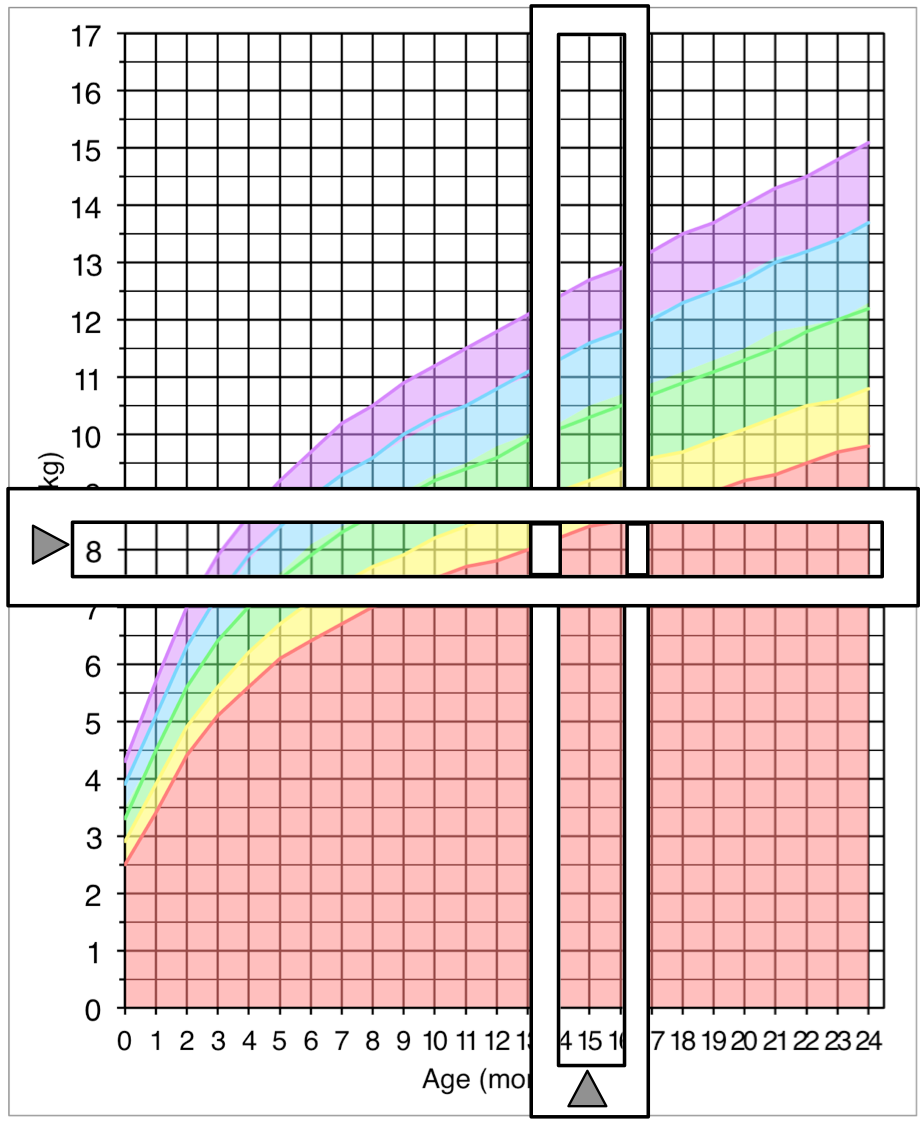
\includegraphics[width=.4\linewidth]{img/graph-strips.png} }}%
    \caption{Different ideas for narrowing focus on a graph.}%
    \label{fig:graph-focus}%
\end{figure}

\begin{figure}%
    \centering
    \subfloat[Baseline slope]{{\label{fig:graph-slope}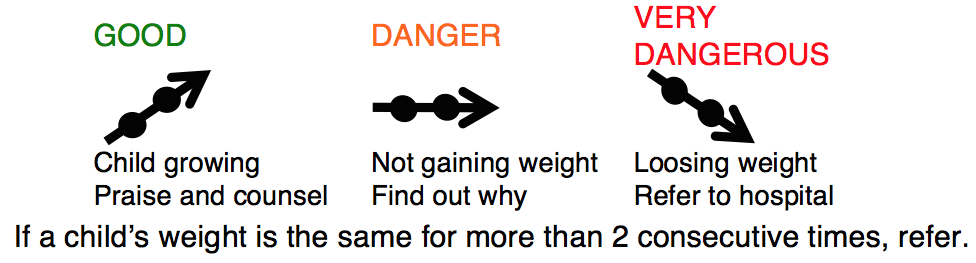
\includegraphics[width=.8\linewidth]{img/graph-slope.png} }}%
    \qquad
    \subfloat[Smart viewfinder]{{\label{fig:graph-viewfinder}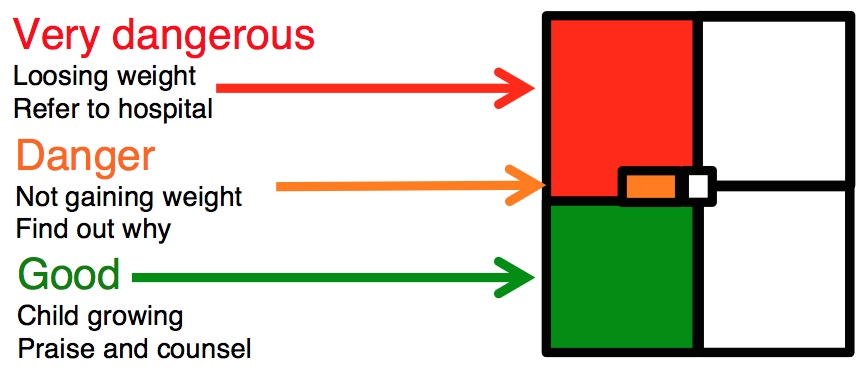
\includegraphics[width=.6\linewidth]{img/graph-viewfinder.png} }}%
    \caption{Different ways of comparing two points to determine change over time.}%
    \label{fig:graph-changein}%
\end{figure}

\subsubsection{Flowchart Booklet}
%JAY: existing flowcharts and final booklet
% JOY: which flowcharts do we want to put? like the ones from grameen from anitha vs. from the chv coordinator (are we allowed to) or the IMCI ones?
Through interviews with a reputable nonprofit organization engaged in public health interventions and interactions with community health volunteers, we learned that one of the tools used by nurses is a decision tree for diagnosing common ailments. This is derived from the Integrated Management of Childhood Illnesses (IMCI), which is a flowchart that instructs the intermediary which questions to ask the caretakers of the patient or which symptoms to check for and how to proceed depending on the results of these inquiries. However, the current representation of the logic for this process is too overwhelming with a lot of detailed information on a single diagram as seen in Figure~\ref{fig:flowchart-grameen} or oversimplifications to accommodate information in a way that is easily represented by a single diagram as seen in Figure~\ref{fig:flowchart-imci}. Therefore, we decided to create a more efficient tool for presenting this information.

We started by simplifying the flowchart so that each potential option would be represented by a different section of the booklet. However, we soon found that this would decrease the amount of space that we would have on the page and detract from our ability to properly show all of the information. So we decided to use tabs to demonstrate the options that a user could take at a given point. After demonstrating our first iterations to an audience of doctors and nurses, it was found that the progress from one step to another was not self-explanatory. Even though the users would follow the steps on the booklet, it was difficult to know when to stop. We tried adding arrows to the pages to indicate the flow from one page to the next, but the arrows were unclear when it came to needing to choose which option to flip. Finally, we found that we would make the options more clear but also to append a long red bar that said ``STOP" at the end of a given action sequence. Since any ``smart" paper tool in a low-resource setting will most likely not come with many user instructions or training sessions, the progression from one step to another has to be fairly clear to the user. The final design for this tool can be seen later in the paper in Figure~\ref{fig:flowchart-booklet}.

% Finally, we also conducted interviews with a reputable not-for profit organization in Accra that was engaged in public health interventions. Through these conversations, as well as through our interactions with community health volunteers, we learned that one of the tools that is used by nurses in the field is a decision tree for diagnosing common ailments. An example is a page on diarrhea treatment from the Integrated Management of Childhood Illnesses (IMCI), which is essentially a flowchart that instructs the intermediary on which questions to ask the parents or guardians  of the patient, or which symptoms to check for, as well as how to proceed depending on the results of these inquiries. However, the current representation of the logic for this process is either too overwhelming in that there is a lot of text on a single diagram, or it is oversimplified in order to accommodate the information in a way that is easily represented on a single diagram. Therefore, we decided to create a more efficient tool for presenting this information to the intermediaries.

\begin{figure}%
    \centering
    % \subfloat[Text-based diagnosis]{{\label{fig:flowchart-chv}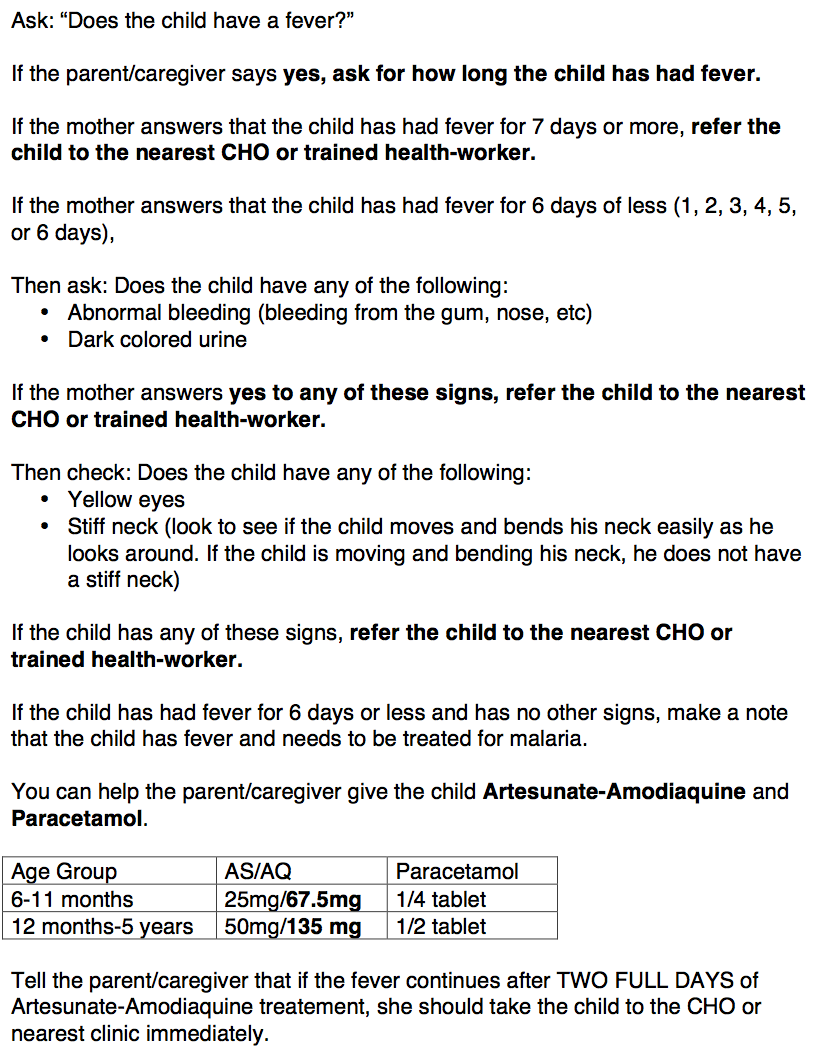
\includegraphics[width=.8\linewidth]{img/flowchart-chv.png} }}%
    % \qquad
    \subfloat[Full flowchart]{{\label{fig:flowchart-grameen}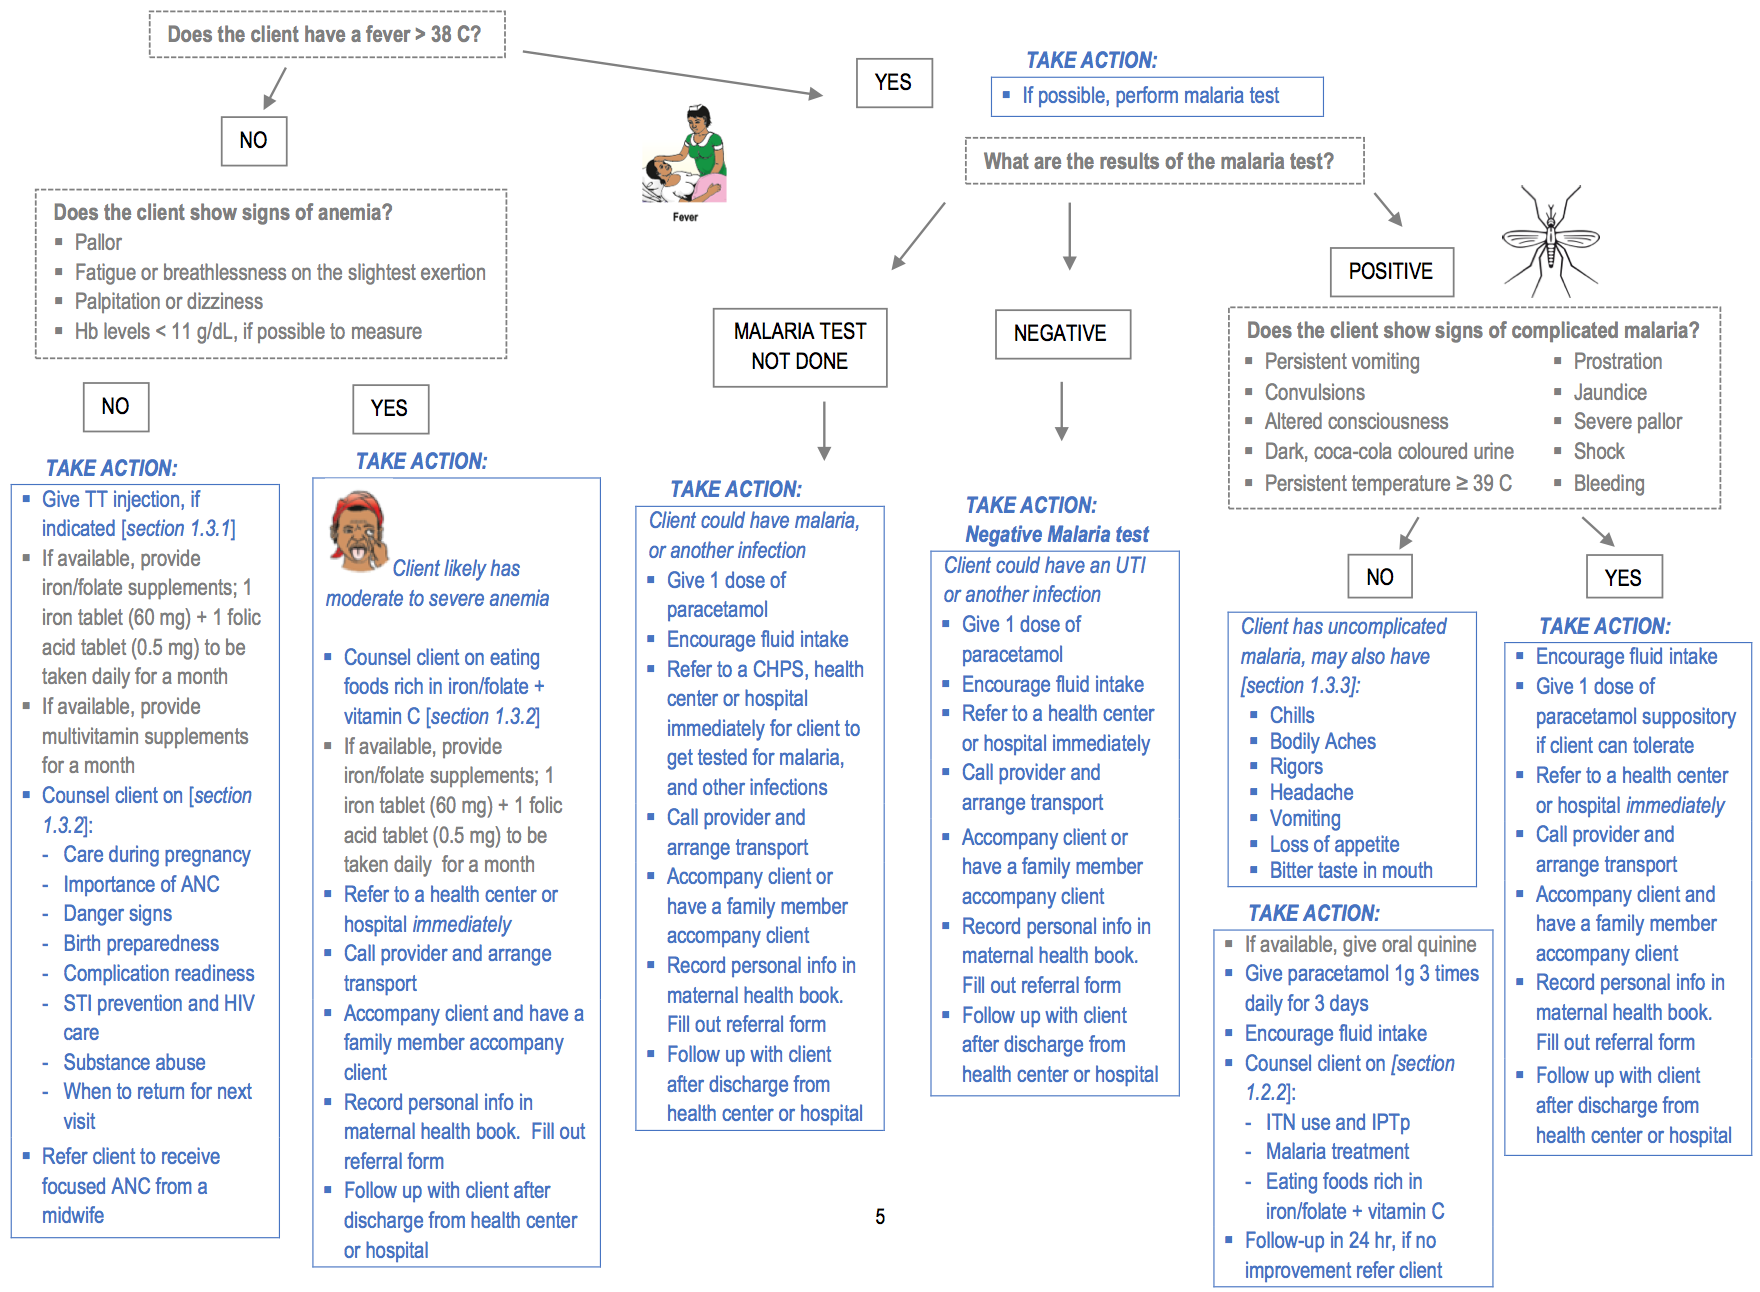
\includegraphics[width=.8\linewidth]{img/flowchart-grameen.png} }}%
    \qquad
    \subfloat[Simplified IMCI flowchart]{{\label{fig:flowchart-imci}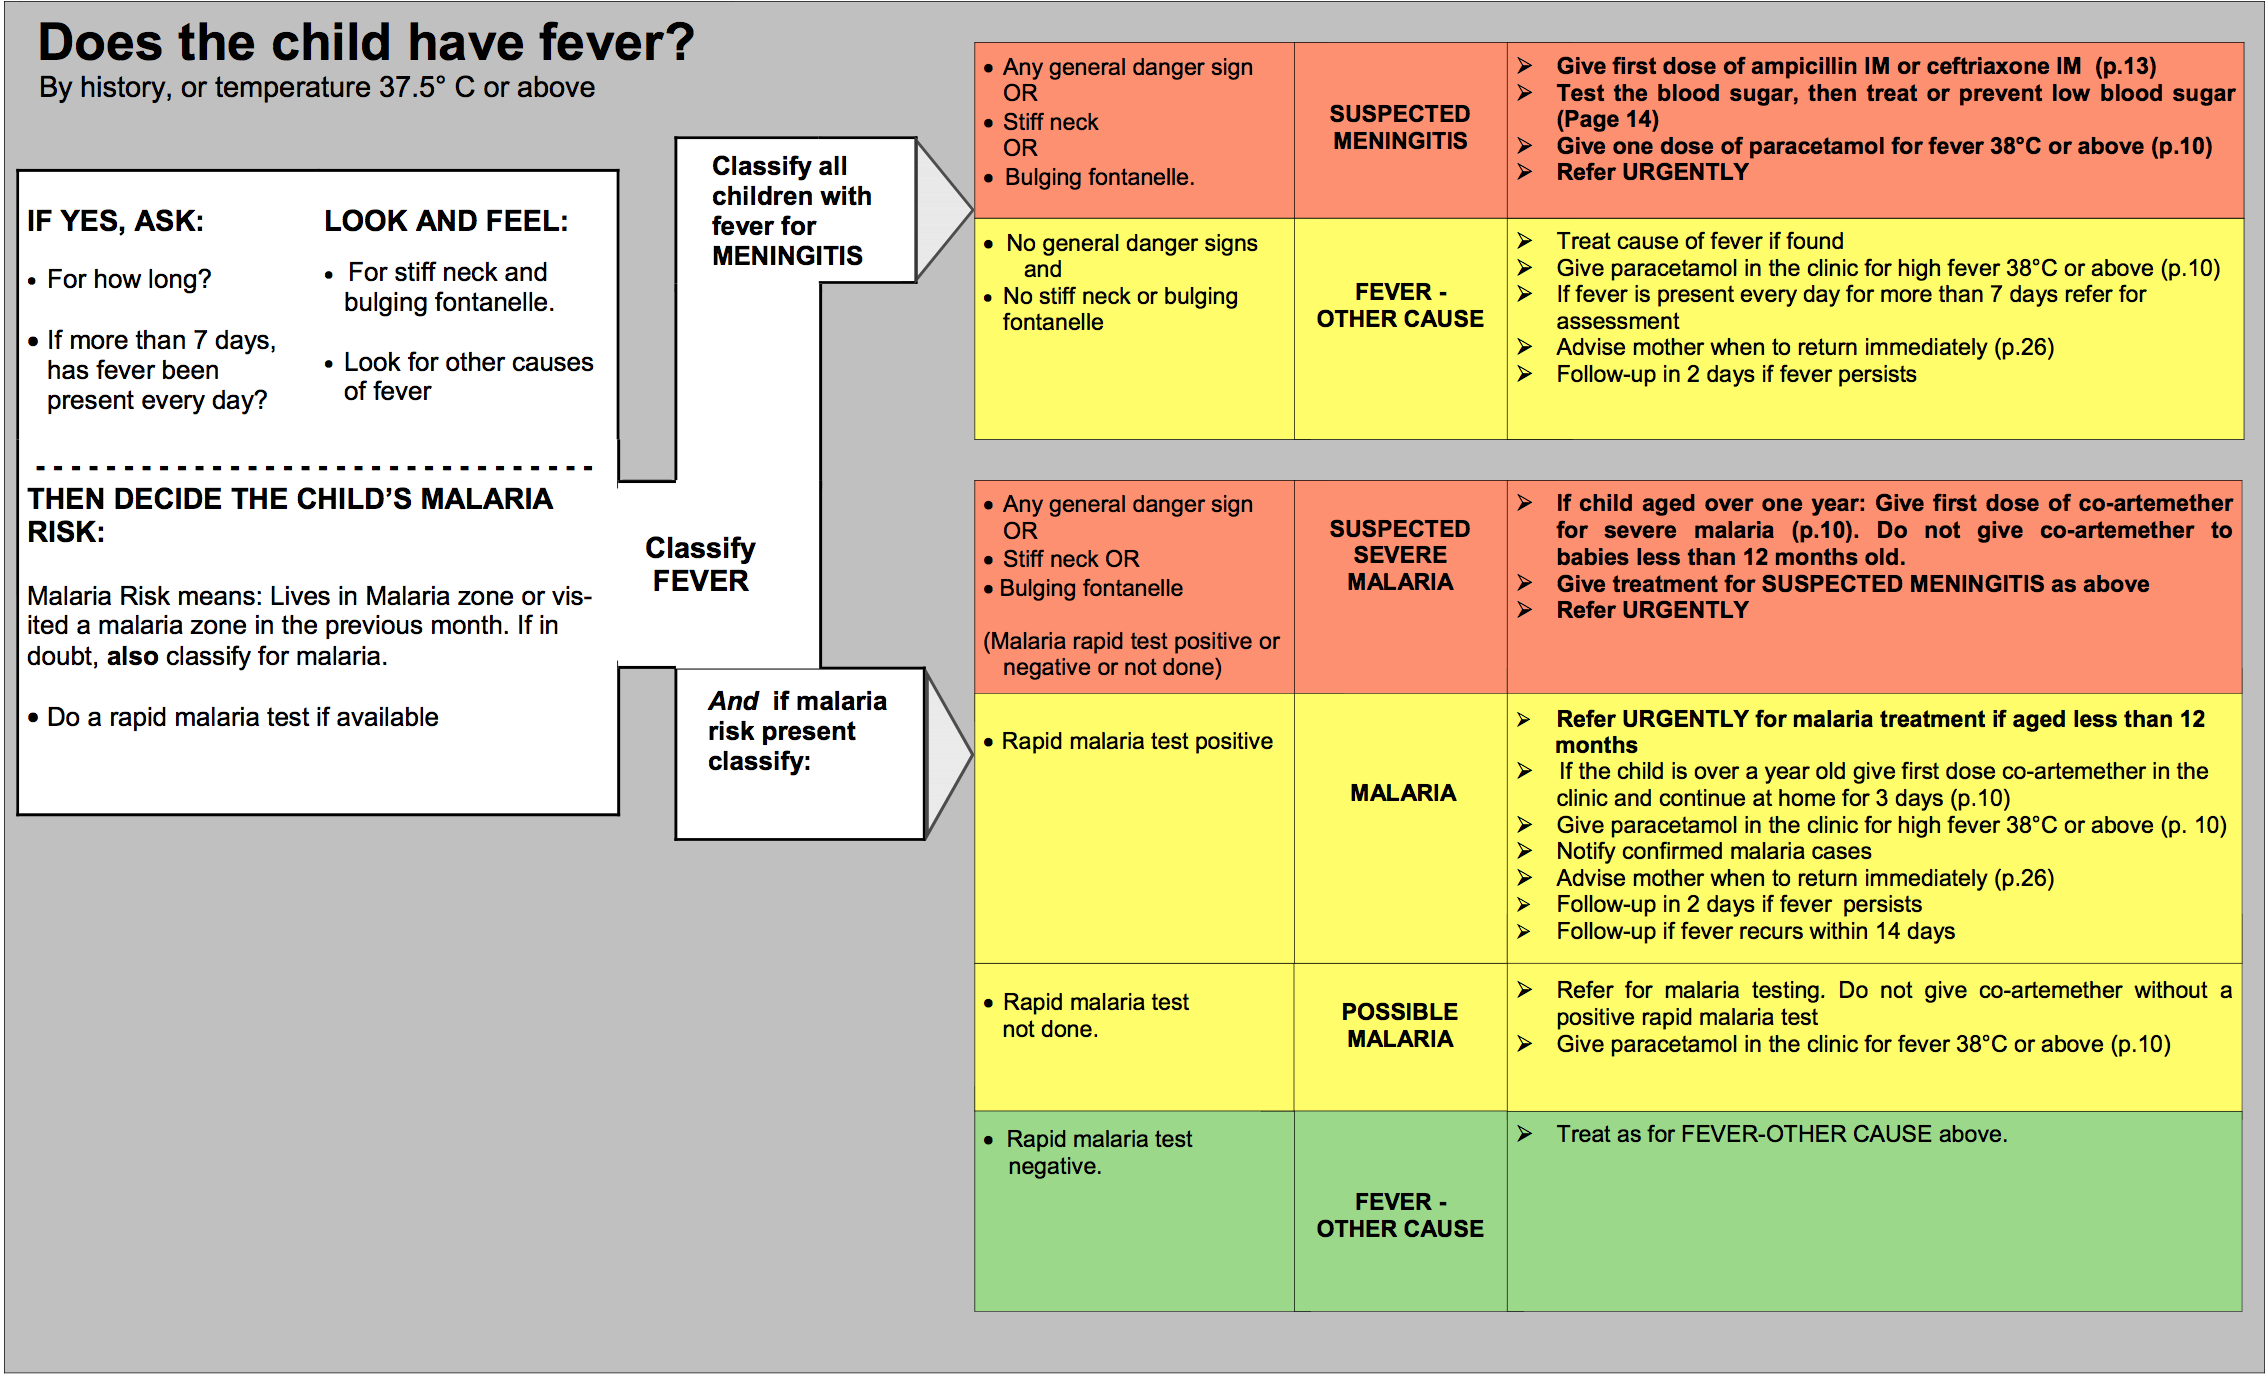
\includegraphics[width=.8\linewidth]{img/flowchart-imci.png} }}%
    \caption{Different flowchart examples.}%
    \label{fig:flowchart-examples}%
\end{figure}

%%%%%%%%%%%%%%%%%%%%%%%%%%%%%%%%%%%%%%%%%%%%%%%%%%%%%

\section{Design}

Given the immense design space of paper-based tools we necessarily had to limit our scope for this project. We reflected upon the paper tools that we encountered and explored in order to abstract our ideas into basic primitives that could be shared across tools. We then considered the various constraints of paper itself, our target users, and our specific contexts to scope the eventual design of \nifty.

%\subsection{Paper Primitives}
%\label{sec:abstraction}

%Reflecting upon some of the paper tools that were encountered and developed, we found that there were some ideas that were common across several of the paper-based tools. For example, both the decision tree tool and the graph reading tool engage different techniques try to narrow the focus so that the end user is dealing with only the information that is relevant to a given scenario. The decision tree tool does so by placing each of the steps or questions on a separate page and the graph reading tool does so by blocking the graph except for the section relevant to the end user. Each of these properties can be traced back towards a more basic aspect of interacting with a two-dimensional piece of paper. In the previous example, both of the tools utilize layering of pages to obscure the irrelevant information and highlight or focus on the currently important information. These aspects such as layering could be considered paper \textit{primitives} that provide specific types of feedback to the user. A list of some examples of primitives and their associated feedback can be found in Table~\ref{table:primitives}.

%\begin{table*}
%\centering
%\caption{Paper primitives and their feedback}
%\begin{tabular}{|p{.35\linewidth}|p{.6\linewidth}|} \hline
%% \being{tabular}{|l|l|} \hline
%\textbf{Primitive} & \textbf{Feedback} \\ \hline
%Color & Highlighting a concept, categorizing an input \\ \hline
%Writing (tallying, words, numbers) & Marking when an event occurs, computation and counting \\ \hline
%Lines & Connecting or comparing two objects \\ \hline
%Circles & Highlighting or focusing on an area \\ \hline
%Shading & Obscuring or hiding, potentially to erase \\ \hline
%Stickers (general placement) & Simulating allocation, tracking when an event occurs, comparing different categories \\ \hline
%Stickers (stacking along one or two axes) & Tracking when an event occurs, computing sums or multiplication/division, comparing computations \\ \hline
%Flipping a page & Demonstrating progress or movement forward, change focus on information \\ \hline
%Layering or stacking (clear) & Computing sums, identifying clusters, demonstrating progress \\ \hline
%Layering or stacking (obscure) & Obscuring other information for focus, subtracting from original \\ \hline
%Splitting pages & Changing focus, allowing for comparison \\ \hline
%Sliding & Changing focus, changing amount, demonstrating progress, juxtaposing different pages \\ \hline
%Reducing size of pages (ripping, cutting, folding) & Decreasing the amount, changing the focus by removing information, creating negative space \\ \hline
%Extending size of page (gluing, taping) & Increasing an amount, magnifying the scope, connecting different pages or concepts \\ \hline
%\end{tabular}
%\label{table:primitives}
%\end{table*}

%From the larger set of the implications of each one of the basic primitives, a smaller set can be drawn, which represents the unique actions paper can contribute to a given task. Some of these actions include categorization or demonstrating progress. Each of these actions could be combined in a paper application as a different \textit{dimension}, representing a different aspect of information. For example, a tool could include stacking of stickers to demonstrate summation and color to distinguish between different categories, covering two different dimensions for categorical tracking. When given a task that needs to be represented by a ``smart" paper tool, the task can be broken down and matched to the different dimensions and primitives associated with them. 

%However, paper only can utilize a finite combination of dimensions at a given time, which constrains its ability to be all inclusive. Some primitives are able to fit better with others and other primitives can distract from one another. For example, flipping the page and sliding the page might result in confusion about which action to do at a given time or one motion might interfere with the other. Additionally, some primitives require more effort than others, so there is a tradeoff between the marginal benefit of an added dimension and the increasingly complicated nature of the tool.

%%%%%%%%%%%%%%%%%%%%%%%%%%%%%%%%%%%%%%%%%%%%%%%%%%%%%

\label{sec:constraints}
\subsection {Paper's Limitations}

While the goal of this project was to manipulate paper's many properties in a way that could augment its computational and visual outputs, we were constantly aware of its limitations:
\begin{compactitem}
  \item Paper has {\bf limited computational feedback} when compared to a computer. As an example, while generating the running total in the susu tracker, we were only able to do so because the intervals were of a fixed value. Therefore, providing a dynamic running total for successive numbers with a variable interval between them would be challenging. 
%Eventually, paper has only so many ``dimensions" that can accommodate the different parameters of a given problem. At the same time, we want to state that the range of tools we designed were limited in the extent to which they truly and completely exploited all of paper's many properties and dimensions.
  \item Paper is also constrained by the {\bf limited amount of physical space} that is available for a specific tool. For instance, the range and the upper limit of numbers in the subtraction band must be directly correlated to the size of the base paper/cardboard sheet the user is willing to work with, and that is not unwieldy and difficult to manage.
  \item Paper has {\bf limitations on physical manipulation}. Paper sheets, of course, can be folded or placed next to each other, in order to provide some dynamic re-sizing capabilities, but physical manipulation such as folding also has its limits with respect to the number of folds possible with paper. Paper can provide sliding or pulling/pushing movements (e.g. in the subtraction band as well as the addition/matching tool), but such movements can be awkward or suffer from wear and tear after repeated use. Comparable, low-cost material substitutes, such as ribbons, may be improve certain problems, but we limit our investigation here to paper.
\end{compactitem}


\subsection {User Constraints}

There were constraints on the tool themselves in terms of how self-explanatory or intuitive they were to the end-user, especially to the low-literate populations that we were targeting. User capabilities can be improved through training and other in-person support, but we limited our investigations to paper tools that required minimal training and intermediation.

During our time in the field and through our interactions with the different users, we also discovered that their goals did not always match the broad goals that we had envisioned for the paper tools. This is not necessarily a user constraint per se, but it did certainly place some checks on the tools we designed and tested in Ghana. For instance, we assumed users wanted more complete and precise results that the susu tracker was providing them. However, in many cases, users were actually satisfied with the current passbooks where they were able to approximate their running total, albeit with some amount of effort. This points to a general inertia towards the learning and implementation of new tools, paper or otherwise. Still, retaining the original look-and-feel of an existing paper tool, something that is more reasonable to accomplish with a new paper tool, like we did with the final iteration of the susu tracker, can help alleviate some of this inertia.

Some of our more sophisticated tools involved too much effort to use, which did not suitably justify the benefit that users were able to glean from them. For instance, the effort invested in using the subtraction band tool may be disproportionate to the benefit that users receive from the tool, especially when their goal is not precision, but is instead a suitably accurate approximation.
For similar reasons, while we discussed many paper tool options that would make use of such actions as ripping paper to show approximations, layering paper to demonstrate an increase in magnitude through thickness, or even origami to solve more complex problems, we did not end up designing or iterating on many of these ideas. We limited our \nifty prototype to support only the subset of primitives that we felt confident could be of practical use for health and microfinance problems we encountered.

%%%%%%%%%%%%%%%%%%%%%%%%%%%%%%%%%%%%%%%%%%%%%%%%%%%%%

\section{Papyr}
\label{sec:system-desc}

\nifty is an interactive system that allows intermediaries working at low-resource organizations to rapidly and automatically generate customized paper tools that give computational and visual feedback. Through a series of questions, the intermediary, as the user of \nifty, specifies a task or tasks. The user is then presented with a set of potential tools generated by \nifty and selects the tool that best suits the resources available and the capabilities of the end user. 

In developing \nifty, our main goal is to link the paper primitives that we extracted into an actual usable system. Considering all of the potential types of tasks, the primitives paper could take on, and tools the system could output, we define three different categories of tasks: tracking, process streamlining, and information lookup. The main distinction is whether the information presented is dynamic. Tracking tasks are those that require user input at given time intervals and the resulting information, such as the sum or regularity of a process, is dynamic. Information lookup tasks are ones where the information is static and minimal user interaction is necessary to discover the information. And finally, process tasks are those that require user input to communicate the current, dynamic situation and determine which information would be shown, but the information itself is static.

\begin{figure}
\centering
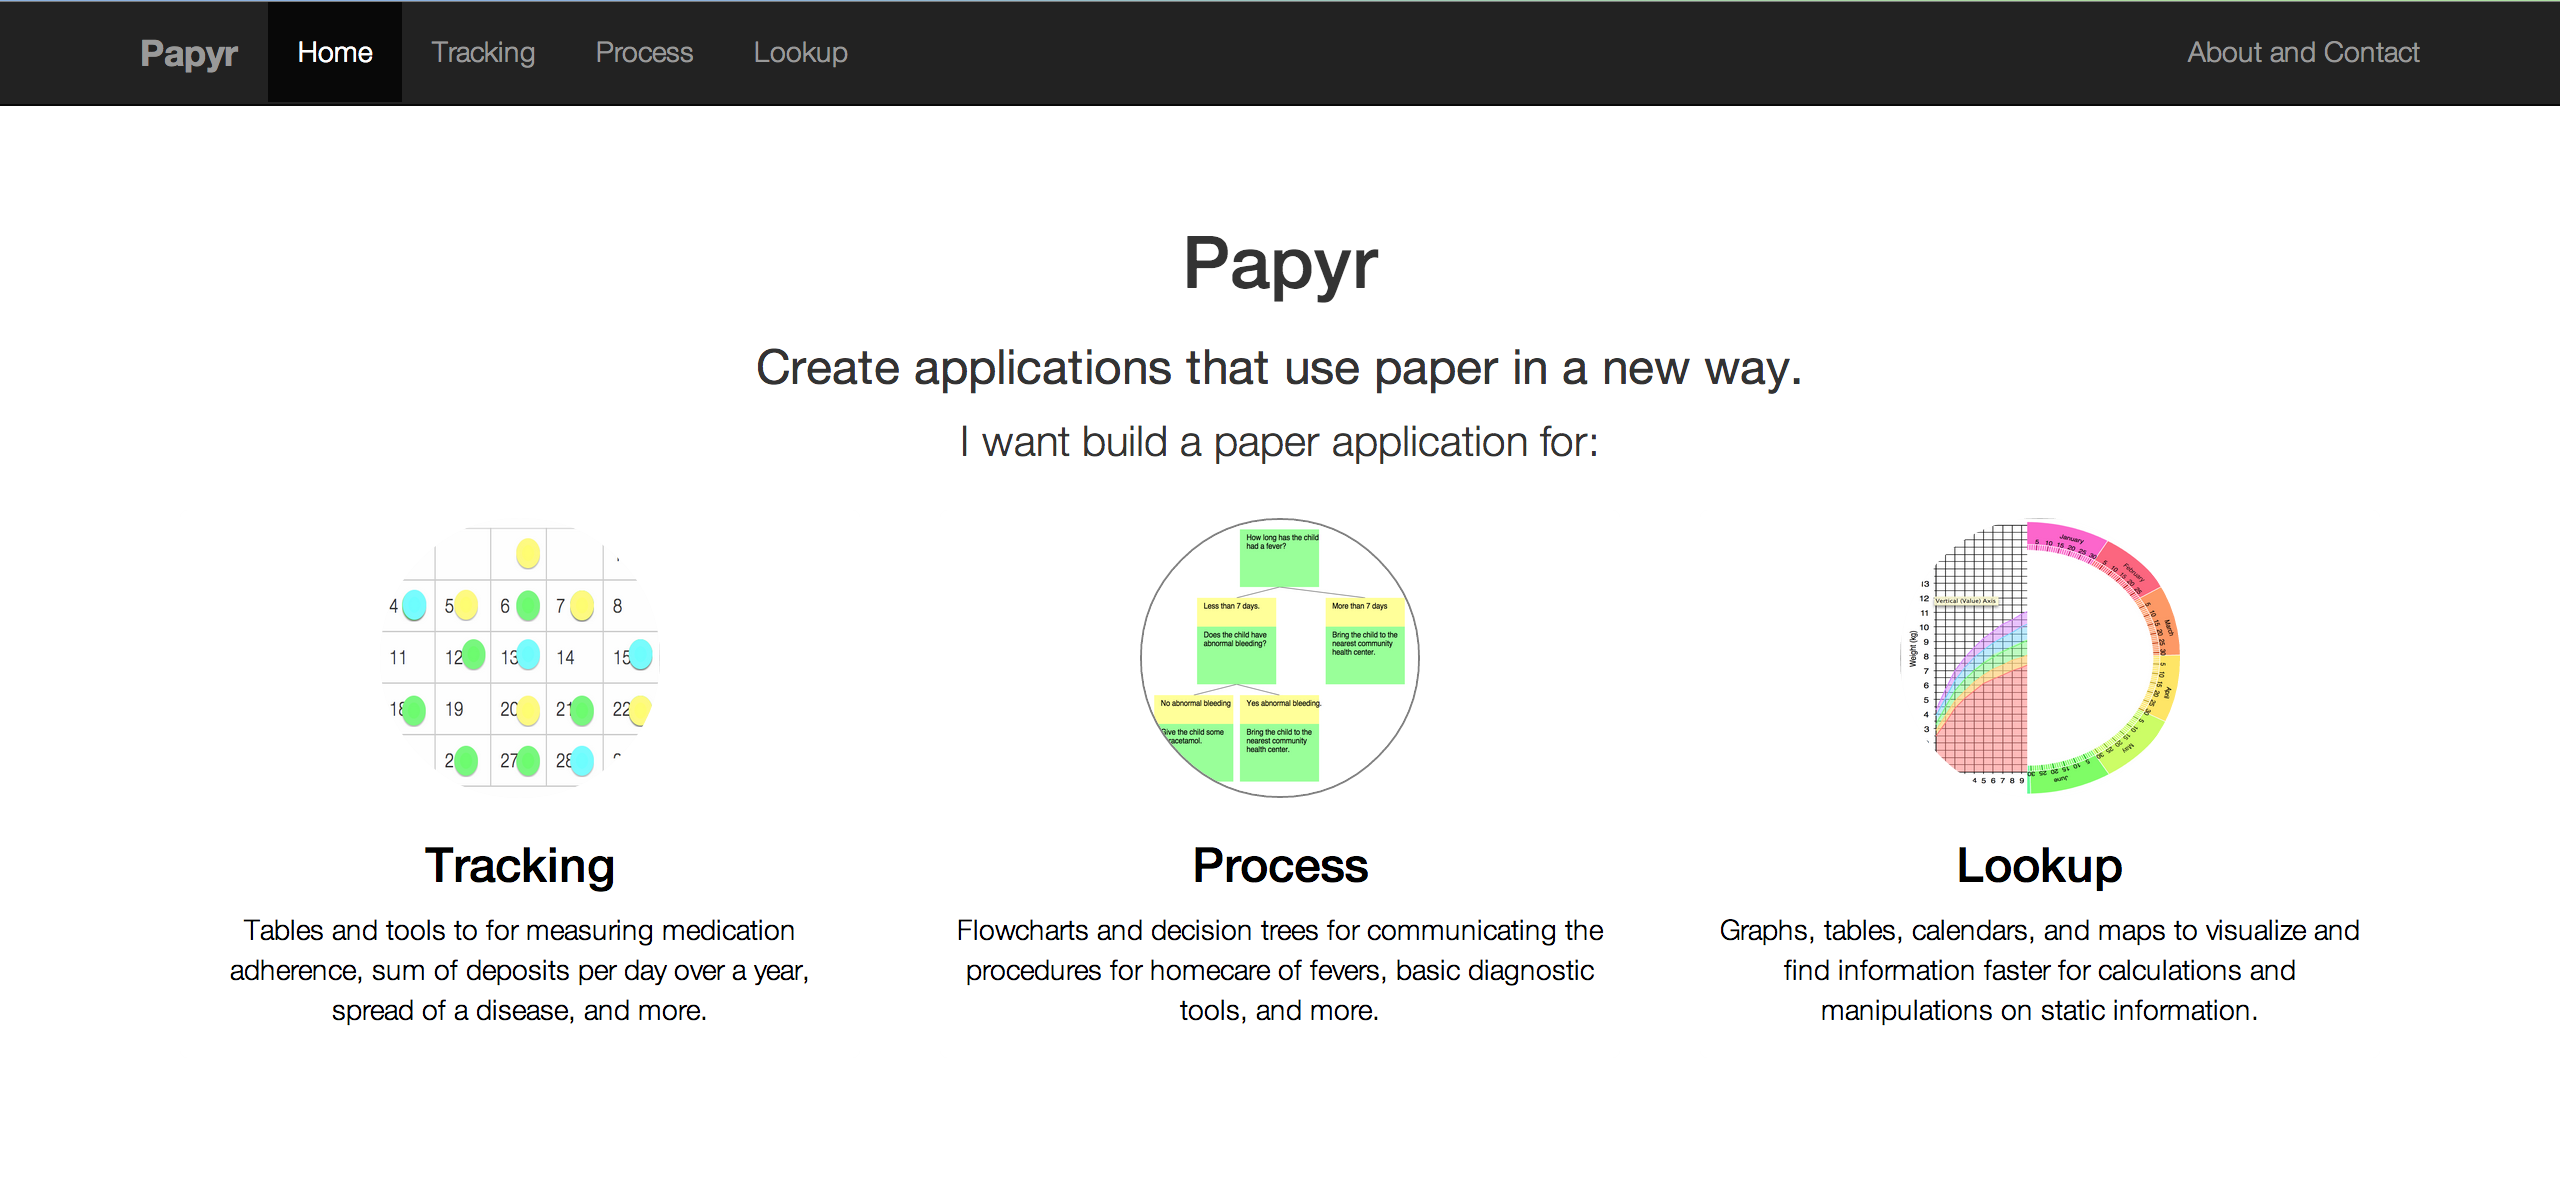
\includegraphics[width=250px]{img/home-screen.png}
\caption{Screenshot of \nifty interface.}
\label{fig:home}
\end{figure}

\subsection{Tracking}

Tracking encompasses tasks that require periodic user input. This includes tracking the days a patient takes his or her pills over a month to visualize the regularity of medication consumption. Alternatively, it also includes tracking the days the microfinance savings customer makes the required two cedi deposits to calculate cumulative sum over half a year. Other use cases include caloric intake each day over a month, amount of sleep each day, length of menstrual cycle each month, mood each day, journaling of events that occur each day, or spread of disease throughout a community over a month.

These tasks all have an element of time and the information achieved relies on this element of time. In the most basic form, each of these tasks can be done using a table. The main dimension of this table reflects the change in time, with each row as a single time interval. This varies for each task based on the frequency and the duration for which the task is tracked. Another dimension is the values in each one of the cells. Some tasks require only a simple yes or no of whether the event occurred to determine regularity, such as medication consumption, and other tasks require a numeric value that could contribute to a cumulative sum, such as daily deposits. 

In the cases where there is more than one piece of data being tracked over time, each task can be defined separately and then, if the time intervals are compatible, automatically merged by our system into a single table with multiple columns. For example, if the task is to track mood every day, and there are five different possible moods, each of the moods is considered a separate tracking task and merged into a single table with one column for each mood. Users can click a checkbox to disable automatic merging of tasks if this is not desired. 
%There are also cases where location is a factor, such as tracking the occurrence of disease throughout a community. This could be construed similarly as many potential categorizations, tracking the occurrence of disease at each individual locale throughout the community.

%Even complicated examples of tracking tasks could be reduced to this basic tracking over time in a table.

The next challenge is allowing users to input task specifications and parameters in an understandable way and to translate this input to paper tool outputs. We originally proposed to allow the user to string together a series of ``per" and ``over" phrases for each relevant time and location to specify their task. For example, an input could read ``I am tracking the regularity of my medication consumption per day over three months." However, this method proves to be fairly ambiguous and difficult for both the user and the computer with more complicated inputs. Eventually, the minimal series of questions was developed to determine the dimensions of the tracking task and differentiate between each of the potential outputs. 

The resulting system asks the user a series of questions about the tracking task they are proposing, including the values of the input and the frequency and duration of the tracking. The system is interactive---for each question, \nifty iterates on the user's answers and outputs suggestions, allowing the user to visualize the impact of each additional constraint. For example, after answering the first question, ``What are you tracking?", the user is presented a blank one-column table where only the first row is filled with the task name. The next question asks about the possible values of the tracking task. If the user indicates that they are tracking only whether the event occurs or not, another suggested output is the same one-column table populated with ``YES/NO" in each row so that the end-user can circle the corresponding word based on the occurrence of the event. The user can very clearly see the incremental difference between the blank table and the new ``YES/NO" table when choosing between the two.

Each of the output suggestions includes the base table that will be used, as well as a set of possible instructions that vary based on the level of literacy of the end user and the cost of any external materials. In the previous example, for the blank table, the user receives potential instructions of writing either ``Y" or ``N" on each of the lines depending on whether the event occurs, shading in the rows for the time intervals the event occurs, or placing stickers in those rows.

The user then has the opportunity to compare all of the possible tools along with their associated instructions and select the one that matches their specific context. A screenshot of the \nifty Tracking workflow is seen in Figure~\ref{fig:tracking}. The potential table-based outputs are similar to Figure~\ref{fig:add-init} and Figure~\ref{fig:band-final} for ``sticker with calendar" and ``no sticker with merged tables" outputs respectively.

% For example, if the user wants to track their medication consumption over a month, they would first be asked ``What are you tracking?" They then are prompted to complete the sentence ``I am tracking..." with ``my medication consumption." At this step, the user will be presented with a table one column and only the task name, or ``my medication consumption" as the first row. Then the user is asked to specify what types of input could be given at each point in the process. The types of inputs that the \nifty system currently supports includes tracking occurrence or a single numeric value each time. In the case of medication consumption, the user will specify that they are tracking ``whether the event happens or not" and be presented with a tables that have ``YES / NO" prepopulated for each row. Other outputs would include a two column tally of the number of times the event occurs and the number of times the event does not occur. And if the user had chosen a single numeric value for each time, the rows would be prepopulated with the cumulative sum for each row. Then, the user would be asked about the frequency and duration for which they will be tracking, allowing the tables to have an additional column that would be prepopulated with the time increments the user specifies. And the user would also be presented with a clock or calendar for tracking. This could be that the user will simply mark the times in which the event occurs. Or the user could place a green or red sticker to better visualize regularity.

% The user is first asked ``What are you tracking?" and will answer "I am tracking my medication consumption." This will output a basic empty table with just Then they will be asked to clarify what values this could take on for each time interval, which, in this case, would be whether the event of medication consumption occurred or not. 

% For example, if the user wanted to track their medication consumption over a month, they would first be asked ``What are you tracking?"
%JAY: 2 examples of questions and final outputs
% At each step, \nifty iterates on the user's answers and output suggestions. These suggestions include the base table that will be used, as well as a set of possible instructions that vary based on the level of literacy of the end user and the cost of any external materials. 
% JAY: example of a set of possible instructions



\begin{figure}
\centering
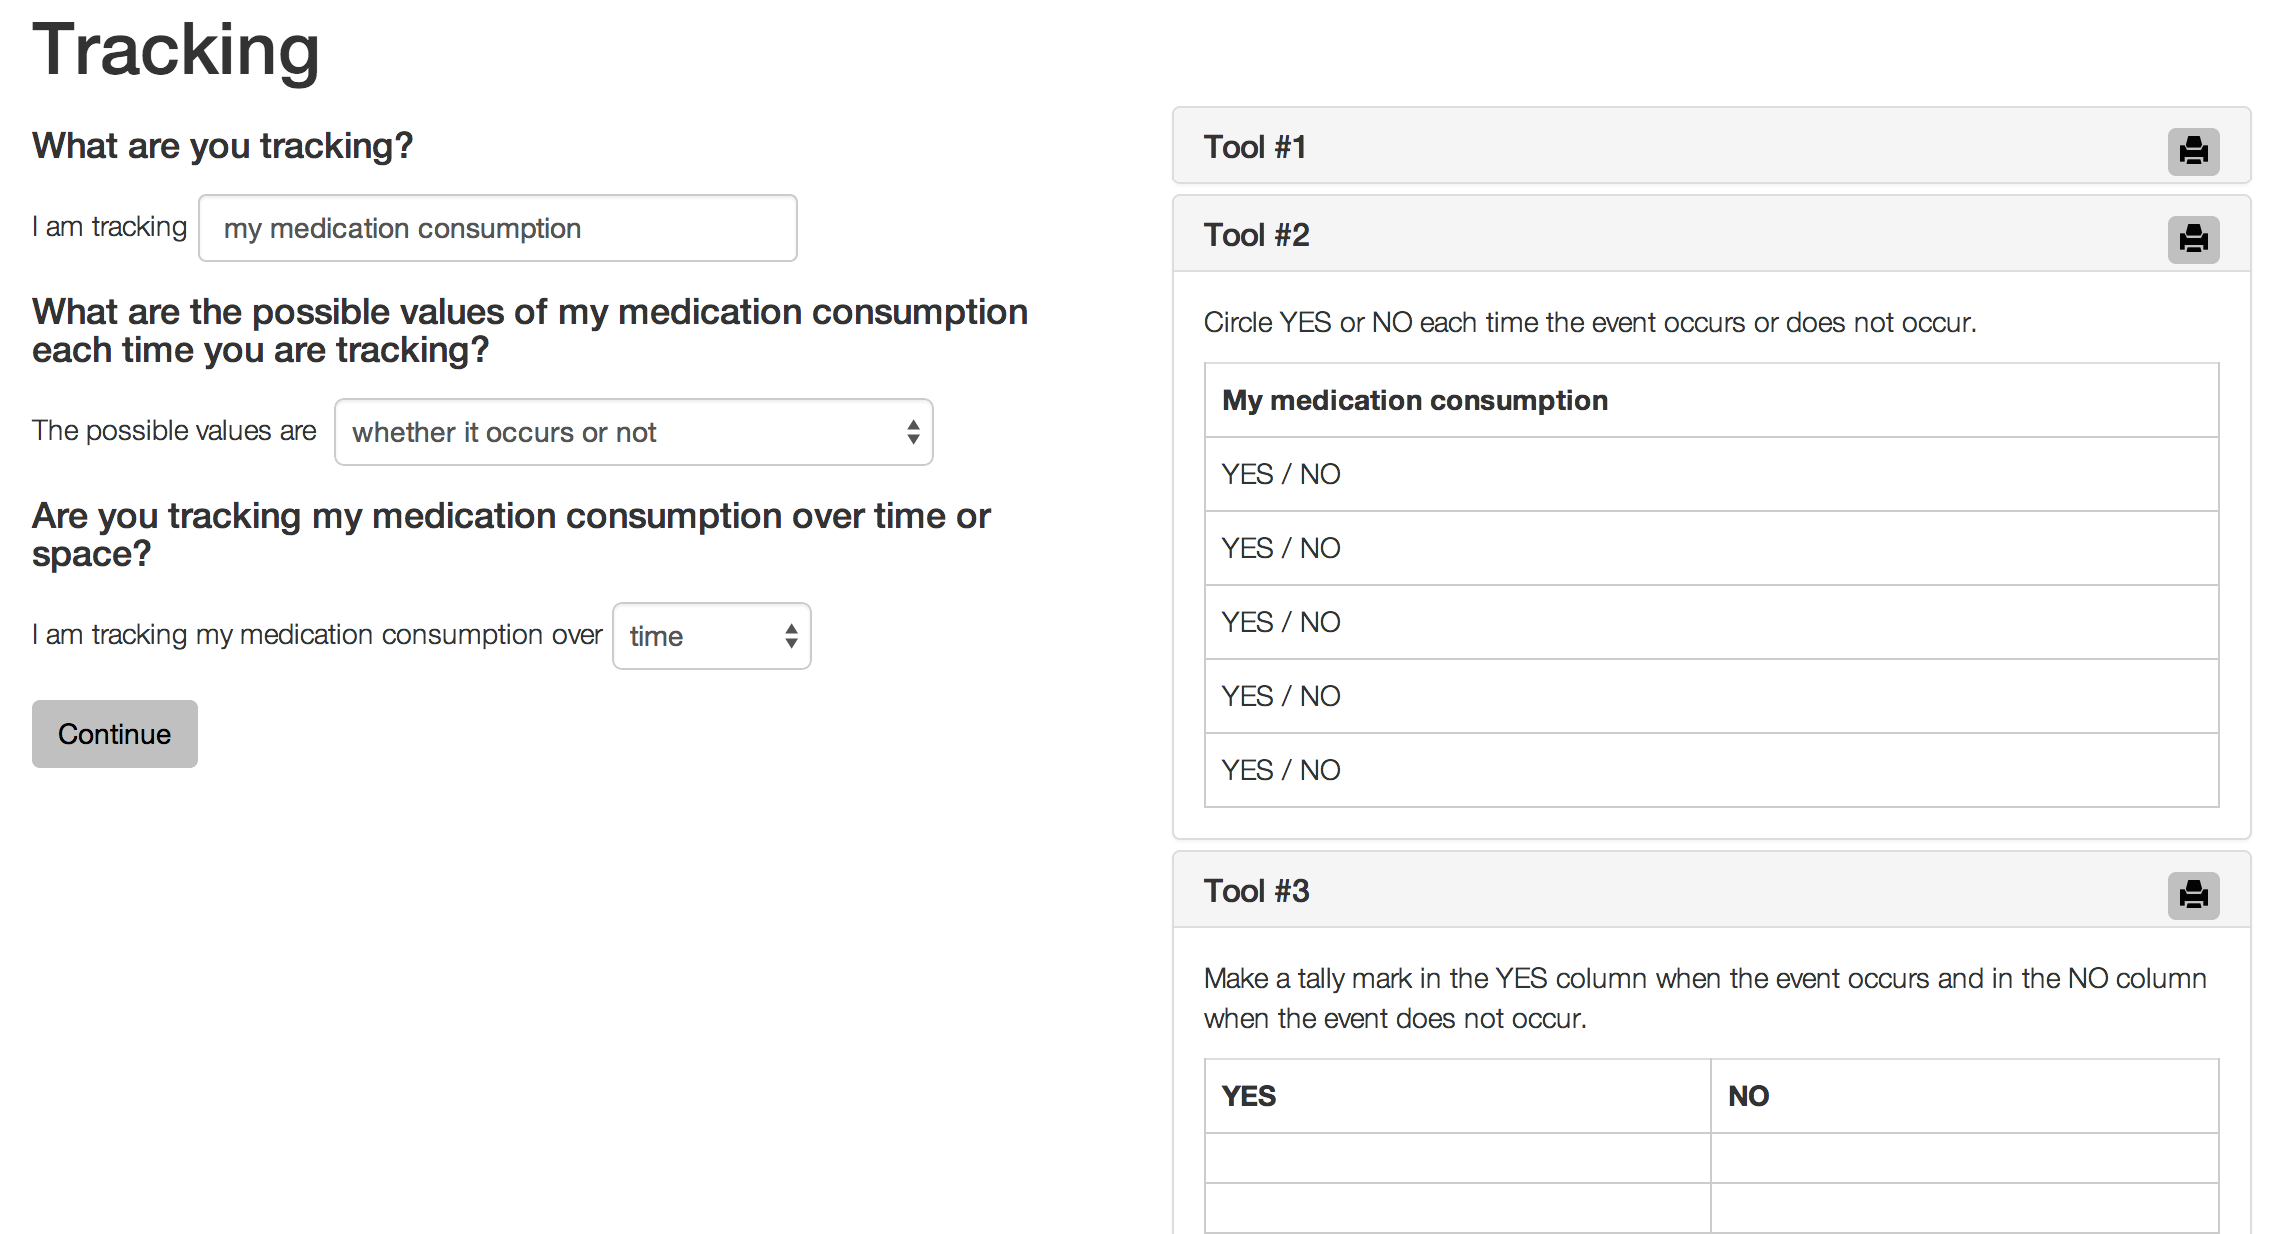
\includegraphics[width=250px]{img/tracking-screen.png}
\caption{Screenshot of tracking interface.}
\label{fig:tracking}
\end{figure}

\subsection{Information Lookup}

While tracking deals with tasks that require user manipulation and input, other tasks deal with static information. These include tasks such as calculating an individual's body mass index (BMI) to looking up whether that BMI falls in the percentiles for being over or underweight. Another would be finding out the number of calories for each food item eaten or checking to see if a child's age and weight are at a healthy balance. The most common forms of static input and output are calculations and information lookups. And in reality, calculations can be construed as information lookups because the answers to a calculation could be enumerated and placed in a lookup table. As with the tracking baseline representation, our baseline representation for lookup is in the form of tables.

The dimensions of these tables are essentially the inputs (i.e. a lookup key) and the outputs (i.e. information the end user is looking up), which are likely numeric or can be reduced to being numerical i.e. categorical). In a basic lookup table, all of the inputs would be in the first columns and the associated outputs would be in the columns that follow, with all possible combinations in each of the rows. This basic layout can be seen in Figure~\ref{fig:table-basic}.

However, there are many cases in which there are more appropriate ways to represent this data than this large, cumbersome table. In a more specific example, where there are two inputs and one output, the inputs and outputs could be arranged such that one input is the columns and the other is the rows and the outputs as the corresponding intersecting cells. This can be visualized in Figure~\ref{fig:table-inputs}. In another case where there are potentially three inputs and one output, a similar row-column structure would work for the presentation of two of the three inputs and the final input would be factored into the separation of the table into tables based on different values for that input. This can be visualized in Figure~\ref{fig:table-split}. And with even larger numbers of inputs, the split could be across different pages, with different colors, and other methods that engage the dimensionality of paper primitives as discussed in the abstraction section.

\begin{figure}%
    \centering
    \subfloat[Basic]{{\label{fig:table-basic}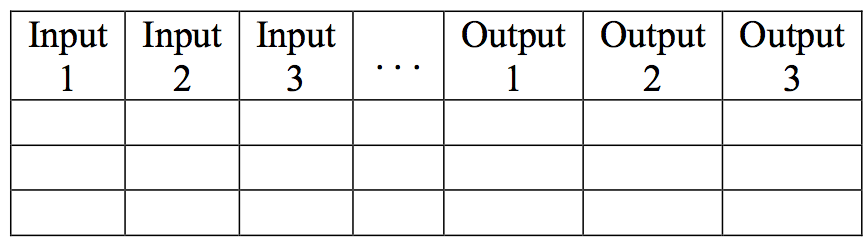
\includegraphics[width=.65\linewidth]{img/table-basic.png} }}%
    \qquad
    \subfloat[Two inputs]{{\label{fig:table-inputs}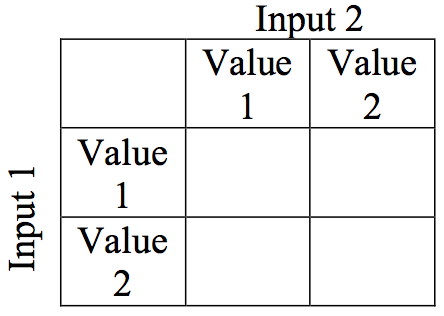
\includegraphics[width=.25\linewidth]{img/table-inputs.png} }}%
    \qquad
    \subfloat[Three inputs]{{\label{fig:table-split}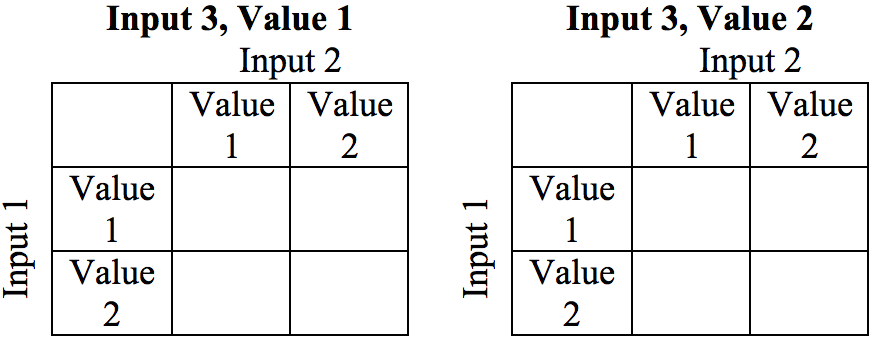
\includegraphics[width=.55\linewidth]{img/table-split.png} }}%
    \caption{Different arrangements of lookup tables.}%
    \label{fig:table}%
\end{figure}

For low-dimensional lookups, tables are relatively easy to use. For higher-dimensional lookup tasks, alternative visualizations are beneficial. A clock or calendar could be used to visualize information that has to do with time or date. Additionally, information could also be presented on a map. Due to lack of space, the two specialized lookup outputs we present here are graph representations and calendar year calculations.

Graph representations cover data that has two numerical dimensions as inputs and a numerical or categorical output. For example, if someone knows their height and weight as numerical inputs, they can figure out whether they fall in the category of under, normal, or overweight based on a graph with those categories as differently colored regions.

\nifty suggests graph enhancements to help end users with understanding the content of the chart or encourage interactivity. These improvements are drawn from the ideas and feedback collected from the graph reading tool we proposed. The first improvement includes tabs and cutouts to help narrow the end user's focus on the relevant region of the graph. For graphs with two axes, this is a vertical sliding cover to isolate based on the y-axis and a horizontal sliding tab to isolate the x-axis. The user can elect to use these components together or separately. This can be seen in Figure~\ref{fig:graph} which shows the output of a graph tool that has the sliding tabs that pinpoint the relevant information to help block out the rest of the graph. 

A second enhancement is a ``smart viewfinder" that guides the end user in doing some basic approximations. For example, sectioning the ``smart viewfinder" into different quadrants in relation to the midpoint helps to determine if the slope of the line from the previous point is positive or negative (e.g. Figure~\ref{fig:graph-viewfinder}). A notched ``smart viewfinder" could help the end-user compare the distance between the two points, whether it is comparing the sizes of bars on a bar graph or the amount needed to increase or decrease to be in a different category or region.

In order to build these graph-based information lookup tools, users will be asked to input the data that they want to work with, and a graph will be built. Then, users will be presented with the pros and cons of each graph improvement and asked which enhancements they want, whether it is the vertical or horizontal tabs or the viewfinder. 

Calendar year calculations are a specific type of calculation for which we developed a paper tool. This tool is made of two concentric circles, the smaller layered on top of the larger. Users can specify the relative number of days between one event and another, provided the difference is within the 365 day range of a year. Then, by spinning the inner circle to line up with a date on the outer ring, the end user can calculate the date of the next event. For example, gestation occurs approximately 280 days after the last menses. A tool for this aligns the 0 day mark with the date of the last menses, the 14 day mark with conception, and the 280 day mark lines up with the predicted gestation day. This sample tool is seen in Figure~\ref{fig:circletool}. To generate this tool for other calculations, the \nifty system takes as an input an indication of which days are matched with which important event in the year range.

\begin{figure}%
    \centering
    \subfloat[Printed]{{\label{fig:graph-print}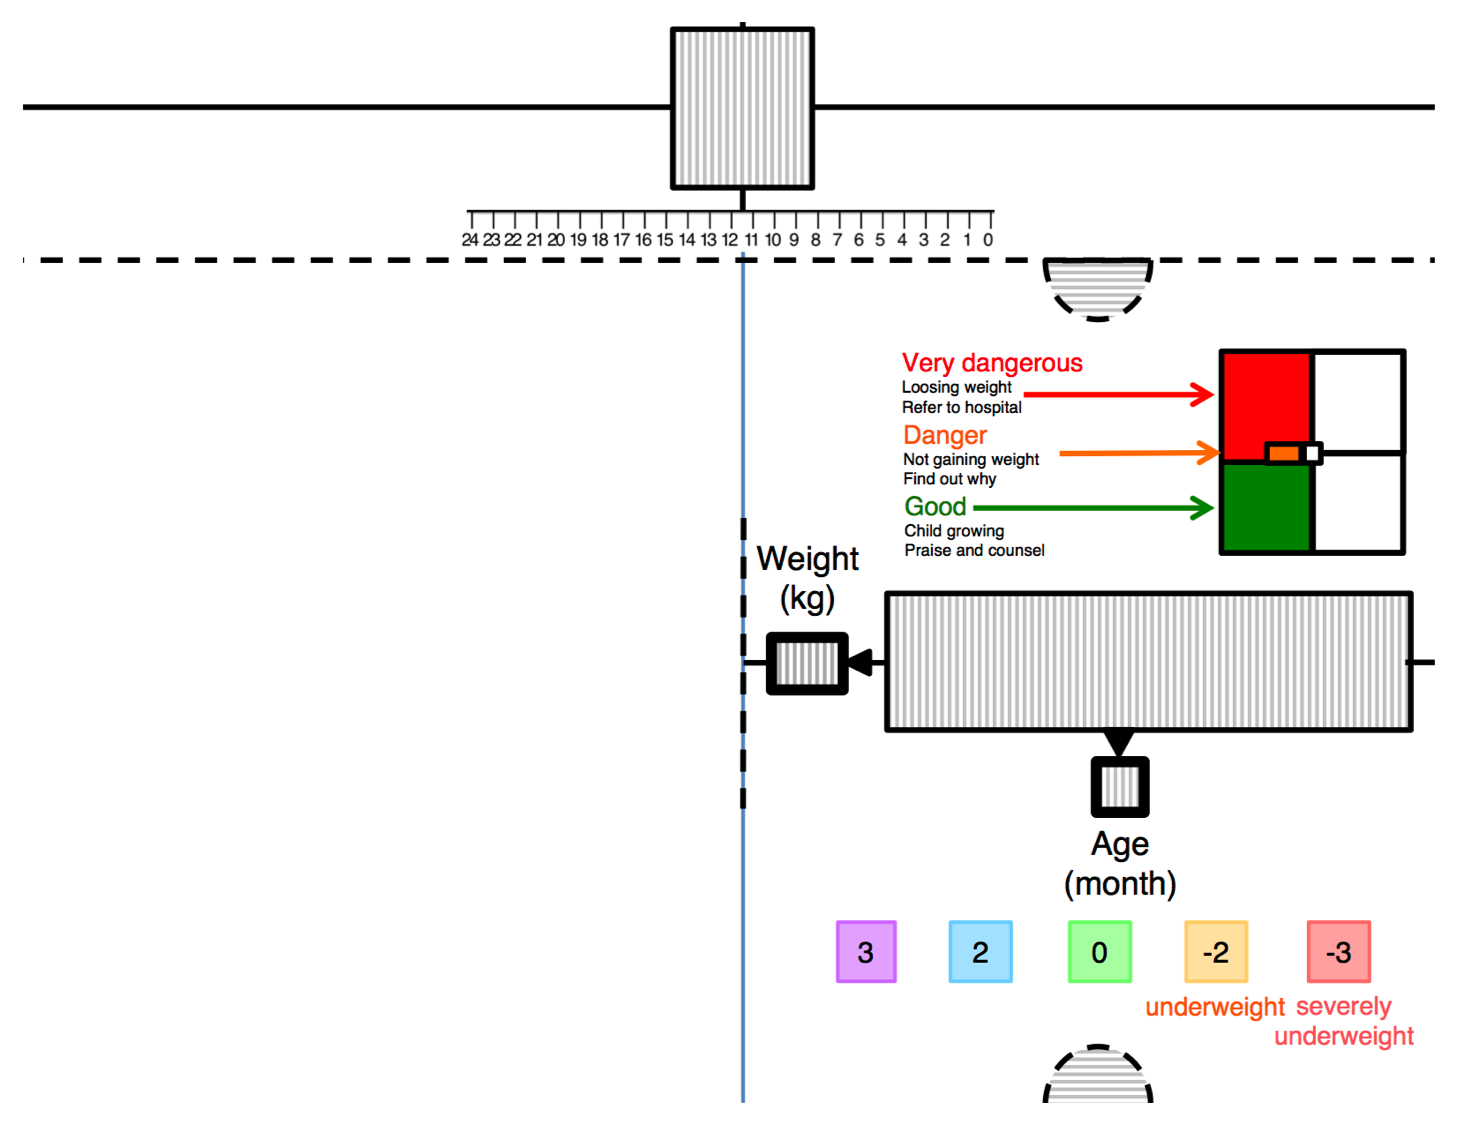
\includegraphics[width=.43\linewidth]{img/graph-print.png} }}%
    \qquad
    \subfloat[Assembled]{{\label{fig:graph-tool}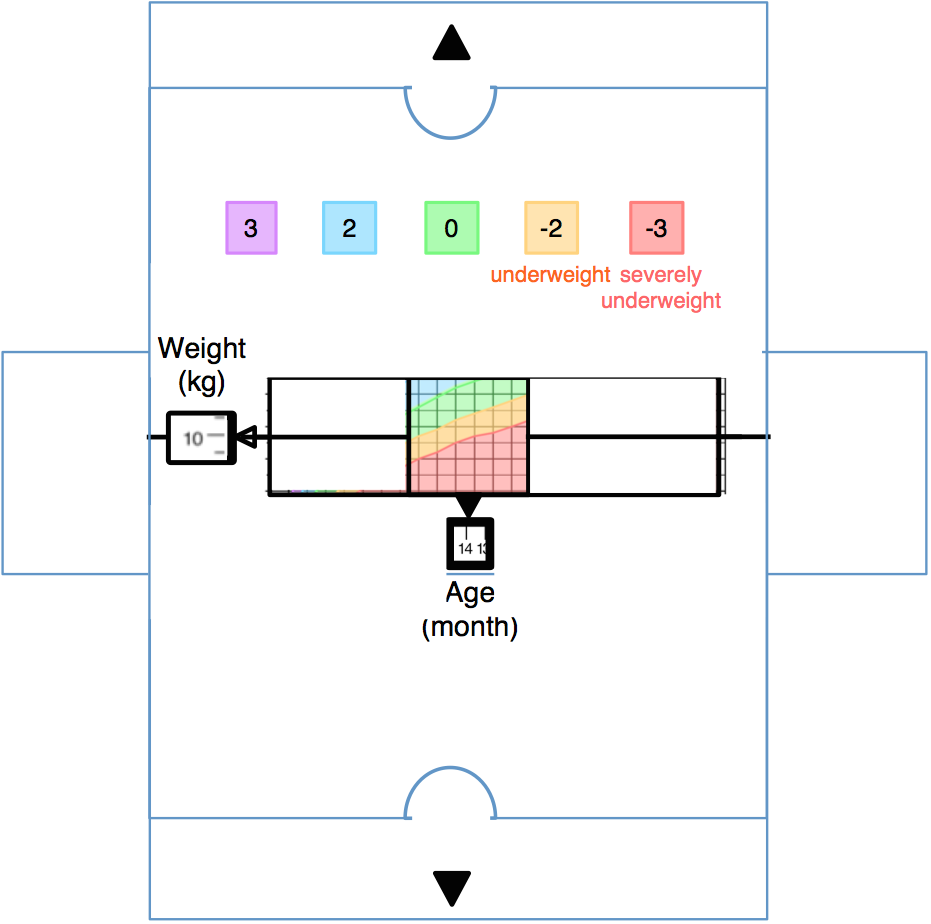
\includegraphics[width=.43\linewidth]{img/graph-tool.png} }}%
    \caption{Output of the graph generation tool printed and assembled.}%
    \label{fig:graph}%
\end{figure}


\begin{figure}
\centering
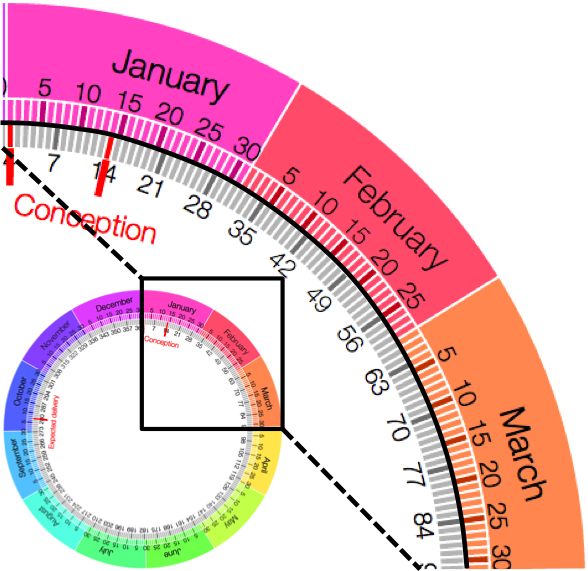
\includegraphics[width=150px]{img/circletool.png}
\caption{Example of calendar year calculation tool.}
\label{fig:circletool}
\end{figure}

\subsection{Process Streamlining}

A specific case of information lookup is process driven---though it has static information, the relevance of this information depends on the specifics of the situation. This information could be presented using a table, with each of the potential factors that contributes to the classification of a given situation as an input and the resulting instructions as an output. However, this would result in a fairly sparse table or many sets of sparse tables separated on different pages or sections. More commonly, this type of information is presented in a flowchart or decision tree. The tool produced by the process module of \nifty can be used to depict this logic, including, but not limited to, questions community health volunteers could use to diagnose a patient, decision diagrams to help a customer choose a savings scheme, or checklists for procedures that change based on the outcome of a step. 

In the \nifty system, the user can specify the logic of the process in flowchart form. The flowchart is a directed, acyclic graph whose nodes are the ``steps" or instructions the end user should follow and whose edges are  ``options" or logical connections from one step to another.

For example, if the user is looking to create a tool to help parents with the home treatment of fever in their children, the user would first create a step with the question of ``How long has the child had a fever?" From this question, there would be two possible paths that can be taken. The user would create another step connected to the first step with the option ``less than seven days" and the instruction to ``bring the child to the nearest community health center." For the other possible answer to the question, the user would create another step that is connected to the first question with the option ``more than seven days" and with the question ``Does the child have any abnormal bleeding?". The user would then continue this process in specifying the answers to this question and continue until no questions remain and all paths end in instruction. This example is presented in Figure~\ref{fig:flowchart}.

Then, the system converts this logic into a booklet. Each page of the booklet will present one question from the flowchart and the potential answer options associated with it as tabs below. The end-user can flip the tab over of the option that they select and continue with either the question or the instruction on the page. An example of the output of the \nifty system is show in Figure~\ref{fig:flowchart-booklet}.

Some of the challenges for this workflow in \nifty include figuring out the order of the steps and instructions. In order to incorporate the feedback from the needs assessment that there should be no blank pages, balanced with the need to show visible instructions, whether it is all possible options at a given time or a ``STOP" instruction, our resulting algorithm for adapting the process logic from a flowchart to a booklet ended up being a depth first traversal that highlighted all nodes, or steps, that were accessed, even those that had been visited before. At each node, the algorithm would access the children of the node and append these options as tabs at the bottom of the page but if there were no children, append a ``STOP". Another challenge was determining the best way to fit all of the instructions on a page, as per the ``screen real estate" constraint of paper. The default presentation of information is using a fourth of an A4 sheet of paper. However, since there seemed to be varying preferences from the feedback, the user also has the option to adjust the size of each of the pages as well and our system uses this to parameterize the output.

\begin{figure}%
    \centering
    \subfloat[Flowchart]{{ \label{fig:flowchart}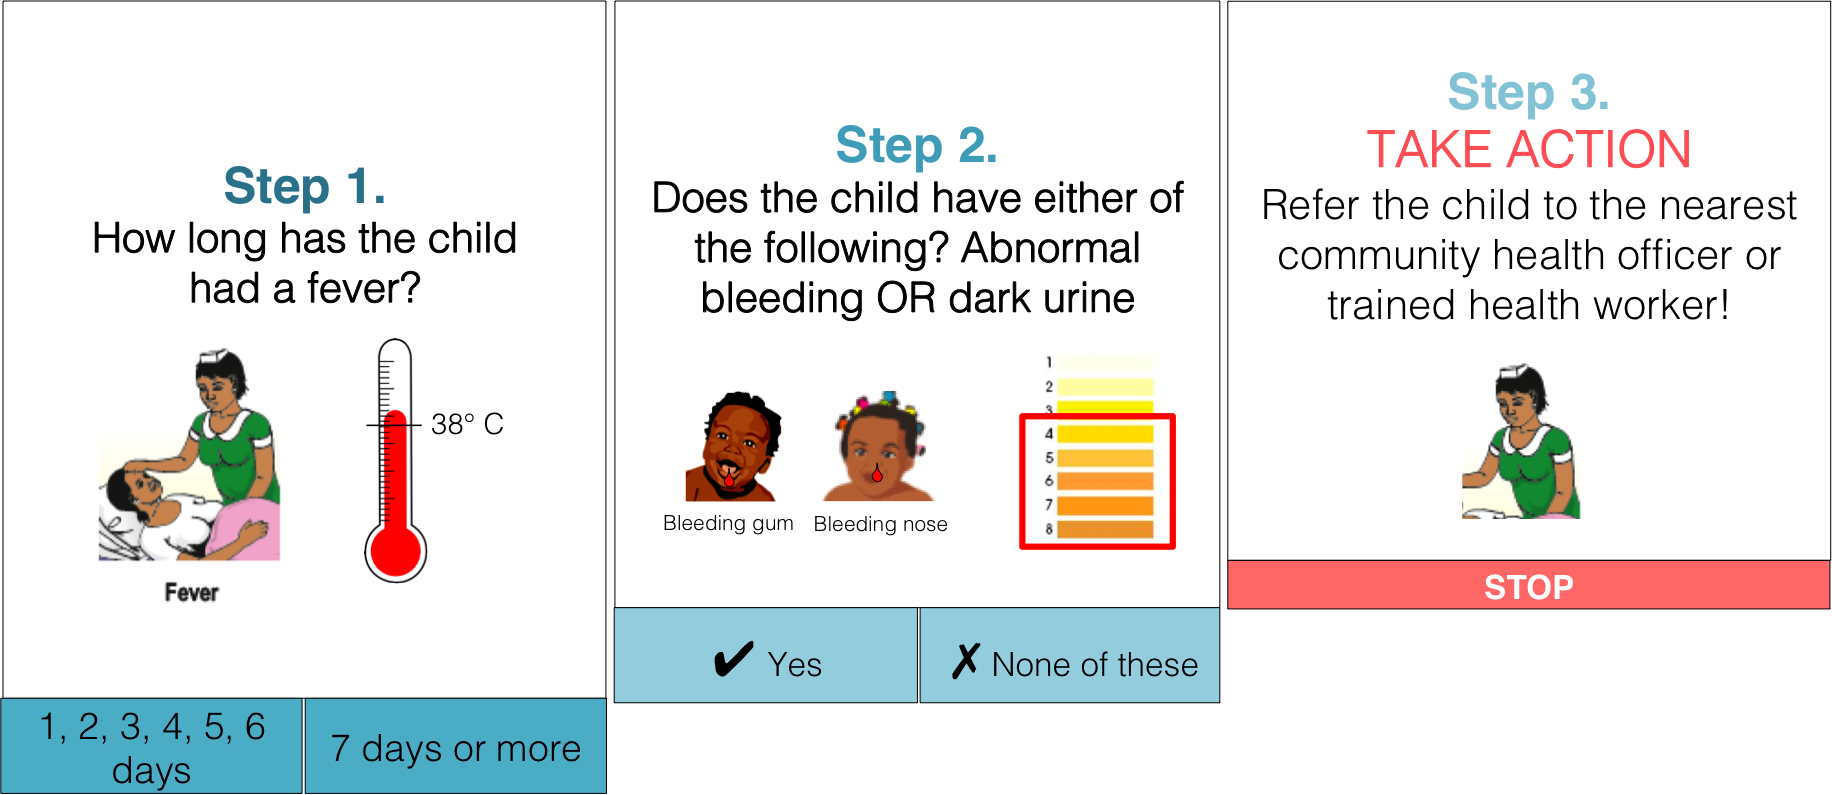
\includegraphics[width=.4\linewidth]{img/flowchart.png} }}%
    \qquad
    \subfloat[Booklet]{{\label{fig:flowchart-booklet}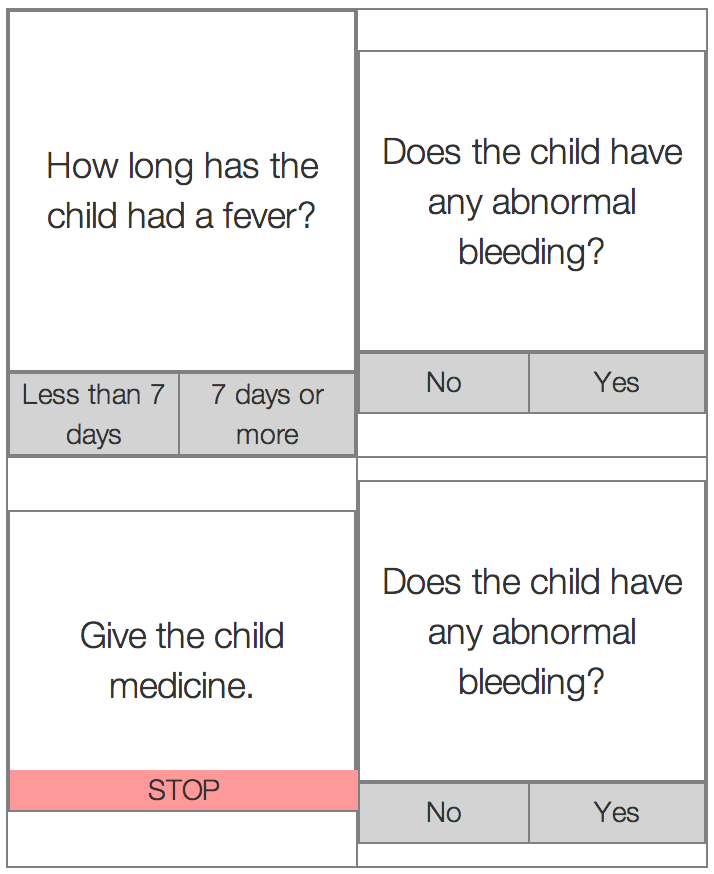
\includegraphics[width=.4\linewidth]{img/flowchart-booklet.png} }}%
    \caption{Process logic depicted as a flowchart and as a booklet.}%
    \label{fig:process}%
\end{figure}

\subsection{Implementation}

The system is implemented as a web-based system with HTML/CSS and Javascript built utilizing the jQuery, Twitter Bootstrap, and D3 frameworks in 2134 lines of code. 


%%%%%%%%%%%%%%%%%%%%%%%%%%%%%%%%%%%%%%%%%%%%%%%%%%%%%

\section{Discussion}
\label{sec:discussion}

The motivation driving this study is the fact that paper is abundant, affordable, deeply embedded in existing workflow practices and personal spaces, and familiar, especially when compared to digital devices that are yet to achieve the same level of adoption and use in the developing world. Furthermore, as we demonstrate in this work, paper is capable of providing augmented computational and visual feedback to achieve some of the everyday tasks that computers currently do. Smart paper can perform basic arithmetic tasks, provide regularity and frequency information through visual feedback, and streamline information dissemination. 

In general, when aiming to solve a problem in a platform-agnostic way (should I use paper or technology?), the design motivations, principles, and applications remain broadly consistent (i.e. without considering technology, all the other design considerations remain the same). Therefore, while working within a given scope, that is the degree of computational or visual feedback required to solve a problem, we encourage a more rigorous and dynamic use of paper to resolve some of these problems, especially in low-resource settings. We believe that the fervent drive to use ICTs to solve a broad range of problems could be scaled back and reconsidered. To avoid the risk of romanticizing paper, we recognize that paper's computational power cannot match that of a computer's. However, paper can certainly be improved over its existing uses as we show specifically in the context of low-resource organizations in public health and microfinance.

\nifty is a supporting infrastructure that automates the creation of the paper tools. \nifty is unlike existing paper computing applications that almost always reduce paper's presence in these applications, diluting some of its more valuable affordances, or replacing it altogether by mimicking its properties in a surrogate (and ``sexy'') technology artifact. Instead, \nifty leverages technology in the design and creation processes, but the output completely preserves the affordances of paper for the end user.

%To better serve the intended audience for the smart paper tools, that is low-literate populations, we define the user of \nifty to be the intermediaries in a given MFI or hospital or other low-resource organization who are better equipped to define the parameters of the tasks that need to be accomplished, and the specific characteristic of the paper tools that need resolution. Moreover, these intermediaries are more likely to have access to the necessary equipment to be able to use \nifty to generate the paper tools. In this way, we distinctly separate the design, development, and the intended audience for \nifty and the smart paper tools it generates.

%Eventually, this paper encapsulates a three month long process of brainstorming, designing, and developing a paper-technology infrastructure that can support the production and distribution of smart paper tools. 
 
%* Paper is abundant, accessible, familiar in low-resource settings. But drawing on paper by hand, or assembling it by hand is tedious and time-consuming. So we introduced a supporting technology infrastructure. However, we believe in paper's independent qualities, and therefore technology is in the picture only up to the point of distribution. 

%* Intermediary uses Nifty Paper, end-user uses the paper tools

%*We demonstrate paper's ability to provide augmented computational and visual feedback. Paper's potential still untapped. Insert commentary about paper's "dimensions"

%* Don't want to romanticize paper. Yet want to make a normative call against productizing at the drop of a hat. Technology does not solve all problems, and going through a resource-intensive process to discover this may be futile. Instead try with paper tools! Insert commentary about how the design process for smart paper tool and technology tools are similar, especially when they are solving the same problem.

%JAY: something about the design space
% Through the survey of existing tools and brainstorming potential tools that push the boundaries of paper, we have discovered some of the principles of designing ``smart" paper tools. 

%JAY: Something similar to this here to contrast again with related work. In contrast,this project focuses instead almost exclusively on exploitingand preserving the valuable affordances of paper by bring-ing in technology to furnish thesupportinginfrastructure togenerate smart paper tools

%%%%%%%%%%%%%%%%%%%%%%%%%%%%%%%%%%%%%%%%%%%%%%%%%%%%%

% \section{Conclusions}

%%%%%%%%%%%%%%%%%%%%%%%%%%%%%%%%%%%%%%%%%%%%%%%%%%%%%

\section{Conclusions and Future Work}
\label{sec:future-work}

This paper describes the an exploration into the design of ``smart'' paper tools in the context of developing regions. We described the process of brainstorming, designing, assessing, and developing a paper-technology infrastructure that automates the production and distribution of smart paper tools. We explored existing paper tool use in healthcare and microfinance in Ghana to understand how paper is currently being used by low-resource organizations to track and disseminate information. From our needs assessment we iterated on several potential designs of enhanced paper-based tools to push the boundaries of paper. We designed a smart paper generation tool that allows intermediaries to specify tasks to quickly and automatically construct potential paper-based solutions that do not require ICTs at the point of use. We describe the design and implementation of our ``smart paper'' prototype, \nifty and demonstrate how it can be used to produce smart paper outputs that preserve the affordances of paper for the end user.

There are many features that we are still incorporating into \nifty and even more areas of improvement. We believe that there is ample potential to leverage paper's tangibility in future work. We plan to explore many of the ideas we mentioned here including: ripping, stacking, layering, or complex folding (origami) with paper. There is also potential to improve the specific modules in \nifty. For instance, future iterations of the tracking workflow will include improved abstractions and optimizations from the given tables, so as to better handle more inputs across different tasks, including optimizations of using maps to track the events across geographical space. In the same vein, future versions of the information lookup workflow will produce more specialized tools including editable calendars and maps. Finally, a future optimization on process streamlining will allow the inclusion of images as components of the steps, for both the questions as well as the instructions and options to better accommodate low-literate individuals. We plan to provide \nifty as a free open-source platform for immediate use by low-resource organizations.
%JAY: insert a DTL hosted URL later.

%%%%%%%%%%%%%%%%%%%%%%%%%%%%%%%%%%%%%%%%%%%%%%%%%%%%%

\section{Acknowledgements}

We thank the participants of our studies for their patience, helpfulness, and valuable feedback.
% We thank David Hutchful at Grameen Foundation for his valuable assistance on the ground.
% We thank the people we interviewed and who helped give us feedback (?)
% Also, how would you even "deeply thank" someone?

%%%%%%%%%%%%%%%%%%%%%%%%%%%%%%%%%%%%%%%%%%%%%%%%%%%%%
\bibliographystyle{abbrv}
\bibliography{ref}

\end{document}